%
\documentclass[12pt,notitlepage]{article}
\usepackage{amssymb}
\usepackage{amsmath}
\usepackage{graphicx}
\usepackage{epstopdf}
\usepackage{pdflscape}
\usepackage[pdftex,dvipsnames]{xcolor}  
\setlength{\marginparwidth}{2cm}
\usepackage[colorinlistoftodos,prependcaption,textsize=small]{todonotes}
\usepackage{xargs}
\usepackage{tabularx}
\usepackage{longtable}
\usepackage{array}
\usepackage{dsfont}
\usepackage{float}
\usepackage{booktabs}
\usepackage{tikz}
\usepackage{marvosym}
\usepackage{multirow}
\usepackage{pdflscape}
\usepackage[hyphens]{url}
\usepackage{setspace}
\usepackage{epigraph}
\usepackage{bm}
\usepackage{textcomp}
\usepackage{diagbox}
\usepackage{bbm}
\usepackage{verbatim}
\usepackage[framemethod=tikz]{mdframed}
\usepackage{subcaption}
\captionsetup[sub]{subrefformat=parens}
\DeclareCaptionLabelFormat{subpanel}{Panel~(#2):}
\captionsetup[sub]{labelformat=subpanel, labelsep=space}

\usepackage{caption}
\usepackage{lipsum}
\usepackage{mathtools}
\usepackage{scalerel}
\usepackage{stackengine}
\usepackage{amsthm}
\usepackage{epsfig}
\usepackage[
  backend=biber,      
  authordate, 
]{biblatex-chicago}

\usepackage[colorlinks,allcolors=blue]{hyperref}
\usepackage[shortlabels]{enumitem}
\usepackage{subfiles} % Best loaded last in the preamble


\setlength{\epigraphrule}{0pt}
\renewcommand{\baselinestretch}{1.25}

\setcounter{MaxMatrixCols}{10}

\newcolumntype{L}[1]{>{\raggedright\let\newline\\arraybackslash\hspace{0pt}}m{#1}}
\newcolumntype{C}[1]{>{\centering\let\newline\\arraybackslash\hspace{0pt}}m{#1}}
\newcolumntype{R}[1]{>{\raggedleft\let\newline\\arraybackslash\hspace{0pt}}m{#1}}



\newcommand{\I}{\mathbb{I}}
\newcommand{\E}{\mathbb{E}}
\newcommand{\Ll}{\mathrm{L}}
\newcommand{\R}{\mathbb{R}}
\renewcommand{\L}{\mathbb{L}}
\newcommand{\Var}{\mathrm{Var}}
\newcommand{\Cov}{\mathrm{Cov}}
\newcommand{\Corr}{\mathrm{Corr}}
\newcommand{\Prob}{\mathbb{P}}
\newcommand{\supp}{\mathrm{supp}}
\newcommand{\notimplies}{\mathrel{{\ooalign{\hidewidth$\not\phantom{=}$\hidewidth\cr$\implies$}}}}
\newcommand{\var}{\mathrm{var}}
\newcommand{\Bias}{\mathrm{Bias}}
\newcommand{\cov}{\mathrm{cov}}
\newcommand{\corr}{\mathrm{corr}}
\newcommand{\MSE}{\mathrm{MSE}}
\let\OldTodo\todo
\RenewDocumentCommand{\todo}{O{} m}{\OldTodo[#1]{\textbf{TODO}: #2}}
\newcommandx{\thiswillnotshow}[2][1=]{\OldTodo[disable,#1]{#2}}
\newcommandx{\askjesse}[2][1=]{\OldTodo[linecolor=Plum,backgroundcolor=Plum!25,bordercolor=Plum,#1]{\textbf{{Ask Jesse:}} #2}}
\newcommandx{\longterm}[2][1=]{\OldTodo[linecolor=Blue,backgroundcolor=Blue!25,bordercolor=Blue,#1]{\textbf{{Long-term:}} #2}}
\newcommandx{\donow}[2][1=]{\OldTodo[linecolor=Green,backgroundcolor=Green!25,bordercolor=Green,#1]{\textbf{{Do Now:}} #2}}


\topmargin=-1.5cm \textheight=23cm \oddsidemargin=0.5cm
\evensidemargin=0.5cm \textwidth=15.5cm

\newtheorem{theorem1}{Special Theorem}

\newtheorem{ass}{Assumption}
\newtheorem{definit}{Definition}
\newtheorem{prop}{Proposition}
\newtheorem{thm}{Theorem}
\newtheorem{lem}{Lemma}
\newtheorem{conj}{Conjecture}
\newtheorem{cor}{Corollary}
\newtheorem{rem}{Remark}

\renewcommand{\thesubsection}{\arabic{section}.\arabic{subsection}}
\renewcommand{\thesubsubsection}{\arabic{section}.\arabic{subsection}.\arabic{subsubsection}}

\newcommand\dapprox{\stackrel{\mathclap{\tiny \mbox{d}}}{\approx}}
\newcommand\papprox{\stackrel{\mathclap{\tiny \mbox{p}}}{\approx}}
\newcommand\pconverge{\stackrel{\mathclap{\tiny \mbox{p}}}{\to}}
\newcommand\dconverge{\stackrel{\mathclap{\tiny \mbox{d}}}{\to}}

\addbibresource{source/paper/references.bib}


\newcommand\independent{\protect\mathpalette{\protect\independenT}{\perp}}
\def\independenT#1#2{\mathrel{\rlap{$#1#2$}\mkern2mu{#1#2}}}

\onehalfspacing
\newtheorem{theorem}{Theorem}
\newtheorem{corollary}[theorem]{Corollary}
\newtheorem{proposition}{Proposition}

\newtheorem{hyp}{Hypothesis}
\newtheorem{subhyp}{Hypothesis}[hyp]
\renewcommand{\thesubhyp}{\thehyp\alph{subhyp}}

\newcommand{\red}[1]{{\color{red} #1}}
\newcommand{\blue}[1]{{\color{blue} #1}}


% required by modelsummary
\usepackage{tabularray}
\usepackage{float}
\usepackage{graphicx}
\usepackage{codehigh}
\usepackage[normalem]{ulem}
\UseTblrLibrary{booktabs}
\UseTblrLibrary{siunitx}
\newcommand{\tinytableTabularrayUnderline}[1]{\underline{#1}}
\newcommand{\tinytableTabularrayStrikeout}[1]{\sout{#1}}
\NewTableCommand{\tinytableDefineColor}[3]{\definecolor{#1}{#2}{#3}}


\begin{document}

\begin{titlepage}
\title{Collaboration in Organizations: Evidence from Open Source Software}
\author{Christopher Liao\thanks{I thank my  advisors Jesse Shapiro and Ali Hortaçsu, Jordan Rosenthal-Kay, James Traina, Noah Sobel-Lewin, Krishna Dasari, Anjali Pullabhotla, Luis Garicano, Josh Lerner, Frank Nagel, Victor Lima, Kotaro Yoshida, Jeff Gortmaker, Ruru Hoong, Ruby Zhang and Matthew Lee Chen, and members of the Harvard Predoc Workshop and the UChicago Honors Workshop for helpful comments and suggestions.}}
\date{\today}
\maketitle

\begin{abstract}
\noindent Placeholder\\
\vspace{0in}\\
\noindent\textbf{Keywords:} key1, key2, key3\\

\bigskip
\end{abstract}
\setcounter{page}{0}
\thispagestyle{empty}
\end{titlepage}
\pagebreak \newpage

\section{Introduction} \label{sec:intro}
\todo[inline]{Things I want to make sure are clear when I'm writing\\
1. Make sure it's clear here that I'm interested in collaboration BETWEEN imp people\\
2. Notes for writing sample- change collaborative to collaborative\\
3. departed contributor- make sure I'm calling it project, not organization
}

\textbf{Paragraphs 1-2: Motivation. After reading these paragraphs a reader in any field of economics should believe that if you answer your research question your paper will make an important contribution.}

A major issue organizations encounter is contributor departures. An organization's problem-solving ability depends on the knowledge of its contributors; hence, departures can not only lead to fewer hands on deck, but also the shrinking of the organization's knowledge base and problem-solving ability. Oftentimes, the more important the departed contributor, the greater the repercussions. One way organizations can mitigate the repercussions of departures is through collaboration. Collaboration can expose contributors to a wider variety of tasks, allowing collaborators to expand their own knowledge base through learning from others and limit how much knowledge an organization would lose following a departure (\cite{hamilton_team_2003}, \cite{rashid_systematic_2019}). On the other hand, collaboration might also lead to investments in team-specific capital that are inaccessible and ill-fitted for the organization's broader objectives post-departure, negatively affecting collaborators (\cite{jaravel_team-specific_2018}, \cite{azoulay_does_2019}).  Moreover, collaboration can also create organizational burdens, as collaboration involves waiting for others which can be time-consuming and detract from the organization's primary focus. An outstanding puzzle is how the benefits and drawbacks of collaboration interact to shape organizational performance following a important contributor’s departure and the situations where one effect may dominate over another. Understanding that is the goal of this paper.

\todo[inline]{I want to rephrase ``Collaboration can expose contributors to a wider variety of tasks, allowing collaborators to expand their own knowledge base through learning from others and limit how much knowledge an organization would lose following a departure" to speak more closely to what I'm examining in the paper}

\textbf{Paragraphs 3-4: Challenges. These paragraphs explain why your research question has not already been answered, i.e., what are the central challenges a researcher must tackle to answer this question.}

There are two major challenges that must be addressed to assess how collaboration affects projects following the departure of an important contributor. First, granular data about organizations is typically inaccessible to researchers. Second, departures and an organization's collaborative nature are both endogenous, which makes identifying their causal effect on an organization difficult. 

I address the first challenge by studying organizational departures using evidence from open source software (OSS) development organizations. OSS is software that is freely available for use and modification, and is considered a public good. OSS is widely used - a recent report found that 97\% of all software included open source code (\cite{fred_bals_six_2025}). Prominent examples of OSS projects include the operating system Linux, the operating system of choice for 96.4\% of the top one million web servers (\cite{w3cook_os_2015})\footnote{Ubuntu, CentOS, Debian, Fedora, SUSE and Redhat are all Linux-based}, and the machine learning framework PyTorch, which is used by 63\% of all organizations training artificial intelligence/machine learning models (\cite{lawson_shaping_2024}). 

Granular OSS development activity is publicly available for research. Moreover, concerns about the repercussions of departures are particularly acute in the OSS community as most contributors are volunteers (\cite{robles_evolution_2005}, \cite{xu_volunteers_2010}) which leads to high turnover (\cite{izquierdo-cortazar_using_2009}, \cite{rashid_systematic_2019})\footnote{This is also a problem in companies that develop OSS. Software developers have an annual turnover rate of 57.3\% (\cite{terlecki_employee_2025}}). Past research has found that departures negatively affect software quality (\cite{mockus_organizational_2010}; \cite{foucault_impact_2015}).

Identifying the causal effect of departures on organizations and the causal effect of collaboration on mitigating the repercussions of departures is challenging because departure and collaboration are choices made by individual contributors and the organization. Contributor departure can occur for personal reasons unobservable to the researcher, such as personal dissatisfaction with the project (\cite{hannon_retaining_2008}, \cite{yu_empirical_2012}) or employment changes (\cite{miller_why_2019}), that may be related to underlying trends in organizational outcomes. Similarly, projects may choose to be more collaborative because collaboration is more conducive to success in their problem environment or contributors happen to enjoy working together. A naive analysis would risk confounding differences in a project's problem environment or  contributor's personalities with the actual effect of collaboration. 

\textbf{Paragraph 5: This Paper. This paragraph states in a nutshell what the paper accomplishes and how. }

In this paper, I leverage data on open source software to identify a set of plausibly exogenous important departures and quantify the effects of these departures on OSS projects. I analyze how pre-departure organizational characteristics and prior collaboration between the departed contributor and other important contributor affect software development activity. Finally, I probe at the underlying mechanisms that drive collaboration's effect and characterize tradeoffs that collaborative organizations encounter prior to departures. 

\todo[inline]{Return to this once I finish the paper. I sholud figure out whether
`` and extend these results to characterize the impacts on downstream business outcomes. " is going in the paper}
\longterm[inline]{Random Forest can help in a few ways:
1) Identifying aspects of organizations that predict not doing poorly post-departure 
2) See if there's a way random forest can explain tradeoffs
3) Random forest will help because it can deal with continuous values in a more systematic way. Right now I'm essentially assuming functional form - can think about how to phrase}

\longterm[inline]{Paragraphs 6-7: Model. Summarize the key formal assumptions you will maintain in your analysis.

Per discussion with Jesse, I can include a model if it makes mechanisms easier to explain. }
% formal model

\iffalse
Paragraph 4 (if I end up having time to write a model): 
Model of hierarchy incorporates cooperation and communication as key features of the hierarchy that affect downstream project outcomes. However, we take these for granted and irl, communication and cooperation can't be taken for granted
\begin{enumerate}
    \item Extent of communication 
    \item Degree of cooperation, overlap (clustering)
\end{enumerate}

Existing theory tells us how organizations adapt their organizational structure and strategy in response to external shocks. However, it doesn't tell us how that adaption depends on existing organizational structure. One example: communication is an integral part of how an organization solves problems, but we don't model how it occurs. Moreover, communication itself also has pros and cons - does it have a positive effect by sharing knowledge or negative effect by creating reliance and thus inhibiting learning?

% See https://www.sciencedirect.com/science/article/abs/pii/S0268401217310095 for a survey of current work
- Doesn't try to separate relationship between structure and departures
- Does not consider the complementarity of organizational structure 
- Research on impact of organizational structures only provides suggestive evidence on the mechanism by which organizational structures have impacts. 
- The focus of research has been on codebase related outcomes or "project survival" as opposed to more relevant outcomes such as usage. 
\fi 

\textbf{Paragraphs 8-9: Data. Explain where you obtain your data and how you measure the concepts that
are central to your study}
I obtain data on OSS organizations and their software development activity from the Github Archive (\cite{github_archive_github_2025}). My paper hones in on a particular type of OSS organization - those developing widely used Python libraries - because data on usage and software version updates is available through the Python Package Index. Python libraries are collections of pre-written software that provide a diverse range of functionality and are essential to software development in Python, the world's most widely used programming language as of July 2025 (\cite{paul_jansen_tiobe_2025}). Focusing on organizations that all develop the same software category also allows me to avoid dealing with differential unobservable trends across different software categories, such as trends in the popularity of different programming languages. The action-level data from the Github Archive (\cite{github_archive_github_2025}) allow me to identify important contributors and track their contribution and departure patterns. 

\todo[inline]{Add to if I end up using other datasets}

\textbf{Paragraphs 10-11: Methods. Explain how you take your model to the data and how you overcome the
challenges you raised in paragraphs 3-4.}

I identify a set of important departures that are plausibly unrelated to unobservable organizational trends by examining the effect of abrupt departures. Abrupt departures occur when an important contributor is highly active for several consecutive periods until their departure, afterwhich they cease to ever be involved in the organization in any capacity. The literature found that abrupt departures tend to be driven by external shocks unrelated to the project, such as job changes or major life events, rather than internal or project-related factors such as declining interest, dissatisfaction, or project wind-down, which typically involve gradual disengagement (\cite{miller_why_2019}). 

I estimate the empirical effect of important departures using an event study design. My observations are at the organization level and the treatment date is the time period of the important departure. The control group consists of not-yet-treated projects that eventually experience a single departure, which guards against bias introduced by unobserved differences between projects that do and do not undergo departures. To simplify the identification of dynamic effects, I restrict the sample to organizations that only ever experienced a single important departure, so that the treatment is binary and irreversible. My primary estimation method is \cite{callaway_difference--differences_2021}, which allows me to estimate dynamic treatment effects robust to heterogeneity in treatment timing and use the full set of ``not-yet-treated'' projects as controls. 

I define ``collaboration” as the rate at which the departing important contributor works alongside other important contributors. Crucially, this metric is defined solely with respect to the departing individual and is therefore orthogonal to broader “other collaboration” measures among non‐departing actors. To guarantee that such dyadic collaboration is possible and projects do not operate in different problem environments, I restrict the sample to OSS projects that, in every pre‐departure period, feature at least two key contributors. I assess post‐departure outcomes conditional on collaboration by stratifying projects into bins based on their collaboration rates.  To address potential confounding between collaborativeness and the treatment effect, I interact these collaboration bins with additional covariates when evaluating post-departure project outcomes.

\todo[inline]{
Do this:
1. show that my measure of collaboration is unrelated to measures of broader organization-wide collaboration. 
2. Among {x, y, z} dimension, projects with collaborative departed contributors are observably similar to projects with uncollaborative departed contributors. 
- Project age at departure time, Forks, stars, departure date, 
}

\textbf{Paragraphs 12-13: Findings. Describe the key findings. Make sure they connect clearly to the motiva-
tion in paragraphs 1-2.}
\todo[inline]{Finish this section }

\begin{enumerate}
    \item Departures matter
    \todo[inline]{a. How do they affect downstream outcomes (releases, downloads)? \\
    b. Do they affect other outcomes as well, such as discussion (issues opened/comments, willingness to contribute (fork))}
    \item Collaboration with the departed does affect post-departure dynamics. Surprisingly, collaborative projects perform worse. 
    \item Involvement matters. The most involved departed contributor belongs to the project whose post-departure outcomes were worse
    \item Collaboration has large positive benefits for the most involved group. This occurs because in collaborative projects, contributors who were already present increase their productivity. 
    \textcolor{red}{
        \begin{itemize}
            \item Why do those contributors increase their productivity? Think about this from the perspective of what this teaches us about organizations
            \begin{itemize}
                \item Is collaboration with the departed contributor indicative of broader, project-specific trends? How: Examine "other collaboration"
                \item How are the important contributor(s) they work with affected? We would suspect these individuals either benefit most (or suffer most)
                \begin{itemize}
                    \item Use this to segway into better understanding what's going on with communication. 
                \end{itemize}
                \item How can I measure whether "collaborators" are learning?
                \begin{itemize}
                    \item Do collaborators tend to work on more problem types (with and without the contributor)? Do they work on a more diverse set of things compared to others in uncollaborative projects? How does this effect change over time. Does this have an effect on outcomes?
                    \item Does a more long-term collaboration help (time)? What about having collaborated on many problems together?
                    \item Do they engage in other forms of responsibility more often, such as reviewing PRs, closing issues, commenting on other's issues? Does this have an effect on outcomes?
                    \item Are they able to do more things independently (either because the departed contributor isn't involved, or becomes less involved) throughout the duration of their collaboration? Does this have an effect on outcomes?
                \end{itemize}
                \item What are the tradeoffs associated with collaboration? Do the tradeoffs affect post-departure outcomes in any way?
            \end{itemize}
        \end{itemize}
    }
    \item Collaboration has large negative benefits for all other involved groups. This occurs because in collaborative projects, contributors who were already present leave. 
    \textcolor{red}{
    \begin{itemize}
            \item Why do those contributors leave? Think about this from the perspective of what this teaches us about organizations
            \item Are the ones who are leaving the important contributor collaborators? 
        \end{itemize}
    }
    \item New contributors are very productive, even more so than existing ones. Why?
\end{enumerate}


\todo[inline]{It would be nice to place a number on "impacts" caused by departure (what's the headline number?)}
% I also want a robustness for departures (that are vs. aren't abrupt) using that departure filtering event study graph

\textbf{Paragraphs 14-15: Literature. Lay out the two main ways your paper contributes to the literature. Each paragraph should center around one contribution and should explain precisely how your paper differs from the most closely related recent work.}

Open source software has long been a topic of interest in the economics literature. In the past, researchers have been interested in why and how people contribute to OSS (\cite{lerner_open_2001}, \cite{lerner_simple_2002}, \cite{hann_economic_2002}, \cite{lakhani_how_2003}, \cite{robert_g_wolf_why_2003}, 
\cite{hertel_motivation_2003}, \cite{krishnamurthy_intrinsic_2006}, \cite{chakravarty_link_2007}, \cite{xu_what_2020}, \cite{wang_monetary_2022}, \cite{conti_incentivizing_2023}), how open source software organizations are structured (\cite{mockus_two_2002}, \cite{crowston_coordination_2005}, \cite{den_besten_allocation_2008}) and what the factors affecting project success are (\cite{mustonen_copyleft--economics_2003}, \cite{fershtman_open_2007}, \cite{comino_planning_2007}, \cite{belenzon_motivation_2008}, \cite{giuri_skills_2010}). There has also been more recent work that has studied the economic impact of open source software on firms (\cite{nagle_open_2017}, \cite{nagle_learning_2018}), its value (\cite{hoffmann_value_2024}) and potential industrial policy (\cite{gortmaker_open_2025}). Work on OSS contributor departures in the economics literature is sparse, although it is a topic of much interest to the information systems and software engineering literature. \cite{rashid_systematic_2019} provides an detailed overview of that literature. There has been extensive work that seeks to understand the prevalence, motivations and ways OSS organizations can mitigate departures (\cite{robles_evolution_2005}, \cite{hannon_retaining_2008}, \cite{westlund_retaining_2008}, \cite{xu_volunteers_2010}, \cite{yu_empirical_2012}, \cite{miller_why_2019}). There is also work on when abandoned projects are revived (\cite{avelino_abandonment_2019}) and how contributors can engage in ``knowledge sharing" behaviors (\cite{von_krogh_community_2003}, \cite{rashid_exploring_2017}) within an OSS organization. Existing literature has found that software quality can be reduced by both contributor departures (\cite{mockus_organizational_2010}) and the presence of newcomers (\cite{foucault_impact_2015}). Past work has also sought to quantify the impacts of contributor departures based off metrics that measure potential damage incurred to the existing codebase by a departure (\cite{izquierdo-cortazar_using_2009}, \cite{rigby_quantifying_2016}, \cite{nassif_revisiting_2017}). The work most closely related to mine, \cite{rigby_quantifying_2016}, has found that the presence of ``successor" contributors who worked on similar tasks to the departed contributor has the potential to mitigate the impact of contributor departures, though there are several important distinctions between their analysis and mine. 
First, this paper examines 92 projects as opposed to 5. Second, I focus on projects that experience one plausibly exogenous departure to avoid confounding underlying project trends with the impact of departure whereas \cite{rigby_quantifying_2016} examines all departures that occur in a project. Finally, whereas \cite{rigby_quantifying_2016} consider hypothetical impacts on a project based on potential damage to the codebase and hypothetical mitigations based on the presence of a successor, I analyze the actual impacts experienced by projects following departures and am able to quantify, using realized outcomes, how factors such as collaboration affect projects post-departure. 
\todo[inline]{Autofill 92}
There is also a large literature on organizational structure and how it affects organizational outcomes (\cite{bloom_measuring_2007}, \cite{brynjolfsson_1_2012}, \cite{ichniowski_7_2012}). However, the work that is most similar to mine actually comes from the literature on innovation that evaluates the impact of premature inventor deaths (\cite{jaravel_team-specific_2018}, \cite{azoulay_does_2019}). The most closely related work is \cite{jaravel_team-specific_2018}, which finds that co-inventor publication activity is negatively affected by premature deaths and that the effects are driven by close-knit teams with extensive experience collaborating. This paper differs in two key ways. First, my unit of observation is an organization, not a team; this distinction matters for several reasons. There are many more individuals in an organization who could both be affected by departure. Moreover, OSS contributors have reputations to preserve that would be damaged if they stopped fulfilling their key duties. One might also imagine that there's a higher ceiling to invention quality than there is to work done in an OSS organization. Second, in my setting, collaboration and contributions are much more visible; I can observe all communication between contributors, which provides more granular measurements of collaboration and examine how individual characteristics of the departed contributor, within an organization, matter. 


\section{Data} \label{sec:data}
\subsection{Data sample}

I am interested in OSS organizations that develop widely used Python libraries - defined as libraries with at least 1000 monthly downloads each month from September 2018 to July 2023. I focus on the subset of organizations whose development data is publicly available on GitHub. 

The unit of observation is an open source software project. In Panel~\subref{fig:dask-home} of Figure~\ref{fig:dask-screenshots}, I show an example homepage for the Github project \textbf{dask/dask}. Each open source software project has contributors who work on problems. Conceptually, a problem consist of at least one of two components: discussion and solution evaluation. To initiate discussion of a problem, a contributor opens an issue, and discussion occurs in the issue thread. Panel~\subref{fig:dask-issue} of Figure~\ref{fig:dask-screenshots} depicts an example issue thread. If a solution is required for a particular problem, contributors will make code changes. The solver can open a pull request (PR) that is linked to a solution and requests others to review their solution prior to incorporating it into the software. Any general subsequent discussion that occurs regarding the pull request occurs in the pull request thread, and any discussion about specific code changes (with references to the code) occur in the pull request thread.\footnote{There are two exceptions. First, sometimes these code changes are implemented without approval. Second, sometimes pull requests are opened without a prior discussion} Solutions consist of changes to the software's codebase. Each change is called a commit. I define an OSS project’s activity within a time period as all activity within a six-month interval—either January through June or July through December of the relevant calendar year and my period of observation spans from 2015 to 2023. Panel~\subref{fig:project-summary-stats} provides further summary statistics on project activity and contributors. All aforementioned data on development activity are obtained from the GitHub Archive (\cite{github_archive_github_2025}), via Google BigQuery.

\donow[inline]{
Provide insight into what a project is like with a table and add other summary stats that may be interesting as I read the paper (don't delete this)
}

\subsection{Departures, Collaboration and Important Contributors}
\subsubsection{Defining Contributor Departures}
I am interested in the departure effects of contributors who worked extensively on code development. I defined the set of contributors who had worked extensively on code development as those with code contributors above the 75th percentile in each period for at least 3 consecutive periods. From this subset, I classify a contributor as “departed” if, after ranking above the 75th percentile of commits for at least three consecutive periods, their activity across all areas (commits, discussion participation, etc) ceases in the immediately following period and remains at that state for all future observable periods. Finally, we subset to projects that only experience one departure to simplify the identification of treatment effects. Finally, I subset to only include projects with at least 2 important contributors (defined in Section~\ref{sec:collab_imp_contr}) and at least 5 pull requests opened in each of the 5 pre periods prior to departure. This leaves me with 92 departed contributors, and hence 92 projects. Panel~\subref{fig:departed-summary-stats} of Figure~\ref{fig:summary-stats} displays the number of contributors left after each successful filtering. 

\todo[inline]{Use autofills for 92 + summary stats table}

\subsubsection{Defining Collaboration and Important Contributors} \label{sec:collab_imp_contr}

I focus exclusively on collaboration between the departing contributor and other important contributors for three reasons related to the OSS community. First, interactions among unimportant contributors are uncommon because they typically aim only to have their own solutions adopted, rather than to engage with the broader community (\cite{hippel_open_2003}). Second, collaborations in which a non-key contributor engages with a key contributor are largely procedural, as important contributors must approve solutions proposed by unimportant contributors, so variation offers little insight into voluntary collaborative behavior. Finally, behavior among important contributor is most interesting in OSS projects because at the individual contributor level, important contributors are vastly more influential in shaping project outcomes (\cite{crowston_core_2006}). Henceforth, when I refer to collaboration, I refer to collaboration between the departed contributor and other important contributors. 

To operationalize collaboration, we must first specify what constitutes an “important contributor.” Prior case studies of the OSS community (\cite{cox_cathedrals_1998}, \cite{mockus_two_2002}, \cite{gacek_many_2004}) have suggested that the structure of OSS projects is akin to a hierarchy or onion, so the concept that there is a wide gulf of importance between certain contributors and others is accepted in the literature. One natural criteria to evaluate a contributor's importance is to base it off how often they are involved in the organization's discussions. To examine the discussions, I follow \cite{crowston_hierarchy_2006} and construct an undirected social network for each time period in which nodes represent contributors and edges record the number of exchanges in issue and pull request threads. If one contributor’s comment follows another’s within the same thread, I treat that as one exchange. For example, the conversation depicted in Panel~\subref{fig:dask-issue} of Figure~\ref{fig:dask-screenshots} would represent two exchanges between the users engaging in the conversation. A contributor is deemed important in period $t$ if, during any of the three most recent periods ($t,;t-1,;t-2$), they are active and satisfy at least one of the following two criteria: their network degree—or number of unique peers they have exchanged messages with—yields a $z$‐score exceeding 1.5 or ranks highest among all contributors, or they are the focal departed contributor under study. 

\subsection{Defining Collaboration} \label{sec:defining_collab}
For a given project $i$ in time period $t$, and problems $P_{i,t} = \{p_{i,t}^1, \cdots, p_{i,t}^{N_{i,t}} \}$ where $N_{i,t}$ is the number of problems faced by project $i$ in time period $t$
\begin{itemize}
    \item Let $C_{i,t}$ denote the set of all contributors to project $i$ in time $t$. We can decompose all contributors into important and other contributors: $C_{i,t} = C_{i,t}^{imp} \cup C_{i,t}^{other}$ 
    \item For each problem $p_{i,t}^k$ you have a set of collaborators $C_{i,t}^{k} \subseteq C_{i,t}^{imp} $ that consists of important ($C_{i,t}^{k, imp} = C_{i,t}^{k} \cap C_{i,t}^{imp}$) and other collaborators ($C_{i,t}^{k, other} = C_{i,t}^{k} \cap C_{i,t}^{other}$)
\end{itemize}
Collaboration occurs in a problem when 2 or more important contributors are both involved. Hence, overall collaborativeness is deined as as 
\begin{equation}
    \mathrm{OverallCollab}_{i,t} = \frac{1}{N_{i,t}}\sum_{k=1}^{N_{i,t}}\mathbf{1}\bigl\{|C_{i,t}^{k,imp}|\ge2\bigr\}
\end{equation}
The collaboration score has a nice decomposition. Let $d$ denote the departed contributor. We can then define $P_{i,t}^d = \{p_{i,t}^{k} \mid d \in C_{i,t}^k, 1 \leq k \leq N_{i,t} \}$ as the set of problems where the departed contributor $d$ is involved and $N_{i, t}^d = |P_{i,t}^d|$ as the number of problems where the departed contributor is involved. 
I can describe the overall collaborativeness as a function of collaborativeness metrics that involve and totally exclude the departed contributor. 
Define 
\begin{align*}
     \mathrm{DepartedCollab}_{i,t} &= \frac{1}{N_{i,t}^d} \sum_{k \in P_{i,t}^d} \mathbf{1}\bigl\{|C_{i,t}^{k,\mathrm{key}}|\ge2\bigr\} \\
     \mathrm{OtherCollab}_{i,t} &= \frac{1}{N-N_{i,t}^{d}} \sum_{k \notin P_{i,t}^d} \mathbf{1}\bigl\{|C_{i,t}^{k,\mathrm{key}}|\ge2\bigr\}
\end{align*}
then we can rewrite $OverallCollab_{i,t}$ as the following
\begin{align*}
    \mathrm{OverallCollab}_{i,t} &= \frac{N_{i,t}^d}{N_{i,t}} \frac{1}{N_{i,t}^d} \sum_{k \in P_{i,t}^d} \mathbf{1}\bigl\{|C_{i,t}^{k,\mathrm{key}}|\ge2\bigr\} + \frac{N-N_{i,t}^{d}}{N_{i,t}} \frac{1}{N-N_{i,t}^{d}} \sum_{k \notin P_{i,t}^d} \mathbf{1}\bigl\{|C_{i,t}^{k,\mathrm{key}}|\ge2\bigr\} \\
    &= \frac{N_{i,t}^d}{N_{i,t}}\mathrm{DepartedCollab}_{i,t} + \frac{N-N_{i,t}^{d}}{N_{i,t}} \mathrm{OtherCollab}_{i,t}
\end{align*}
Henceforth, most collaboration-related analyses will focus on $\mathrm{DepartedCollab}_{i,t}$

\section{Methods} \label{sec:method}
\subsection{Estimating the impact of departures} \label{sec:main_method}
Denote by $G_i$ the first period where project $i$'s departed contributor is no longer part of the project. Accordingly, project $i$'s treatment indicator at time $t$ is defined as
$$
D_{i,t} = \mathbf{1}\{t \ge G_i\}.
$$

My primary outcome of interest $y_{i,t}$ is the number of pull requests opened by project $i$ in time period $t$. I focus on pull requests because they're the most direct measure of production effort that projects are engaging in. I transform the outcome into a z-score to enable cross-project comparisons under one unit - standard deviations - in spite of underlying cross-project differences in the number of pull requests opened. To avoid contaminating treatment effect estimation, I standardized based on the pre-treatment mean and standard deviation, calculated using the 5 periods prior to treatment.

Define a cohort $g$ as projects with the same treatment date $g = G_i$. For all $t \geq g$, I define the group‐time average treatment effect as 
\begin{equation} \label{eq:group_time}
\mathrm{ATT}(g,t) = \mathbb{E}\bigl [ y_{i,t}(1)-y_{i,t}(0)\mid G_i = g \bigr ].
\end{equation}
Let $k = t - g$. Our primary estimate of interest, the average effect \(k\) periods after departure is
\begin{equation}\label{eq:event_study_time}
\mathrm{ATT}(k) =
\mathbb{E}\bigl[y_{i,G_i+k}(1)-y_{i,G_i+k}(0)\bigr] = 
\sum_{g} \Pr\!\bigl(G_i = g \mid G_i + k \le T\bigr)\,\mathrm{ATT}\bigl(g,\,g+k\bigr).
\end{equation}

My estimation does not involve covariates so the overlap assumption from \cite{callaway_difference--differences_2021} is not relevant. Treatment is irreversible, by definition of $D_{i,t}$ and I assume that $\{Y_{i,1},\dots,Y_{i,T},D_{i,1},\dots,D_{i,T}\}_{i=1}^n$ are independent and identically distributed. Hence, identification of $\mathrm{ATT}(g,t)$ (and hence $\mathrm{ATT}(k)$) requires the following assumptions:\\
\textbf{Limited treatment anticipation}: There exists $\delta\ge0$ such that for all $t<g-\delta$, $\mathbb{E}[Y_{i,t}(g)\mid G_i=g] = \mathbb{E}[Y_{i,t}(0)\mid G_i=g].$\\
I assume no treatment anticipation ($\delta=0$) in my setting, as I am analyzing abrupt departures that are more associated with factors unrelated to project outcomes such as a job or company change. It's worth noting that the full process of a job transition, from giving notice to finding a new job, can occur within the six month window that constitutes a time period in my analysis, especially given the healthy labor market experienced by tech companies over the past decade.\\
\textbf{Parallel trends based on ``not-yet-treated" groups and no anticipation}. For each $g\in\mathcal{G}$ and each $s, t$ such that $g \leq t \leq s$, we assume \[\mathbb{E}\bigl[Y_{i,t}(0)-Y_{i,t-1}(0)\,\bigm|\,G_i = g\bigr] =  \mathbb{E}\bigl[Y_{i,t}(0)-Y_{i,t-1}(0)\,\bigm|\,D_{i,s}=0,\,G_i > g\bigr]\]

The parallel trends assumption states that in the absence of treatment, treated projects would have experienced the same outcome evolution as not-yet-treated projects. 
There are two reasons why I believe the parallel trends assumption is plausible in my setting. First, the analysis uses ``not-yet-treated'' projects as controls, which makes it more likely that underlying, time-invariant factors that differ between eventually treated and never-treated projects do not confound the analysis. 

Second, my analysis focuses on abrupt departures, which survey evidence from \cite{miller_why_2019} shows is associated with ``some kind of transition (e.g., switching jobs or leaving academia)" or because of contributors were ``having children or getting married." Switching jobs or leaving academia increases the difficulty of contributing to OSS because new jobs may not support contributing to OSS or incur additional demands on one's time that take time away from contributing to OSS. These are also departure reasons that are unrelated to unobservable project factors, such as declining outside interest or personal dissatisfaction, which could cause parallel trends violations. Finally, \cite{miller_why_2019}'s focus on abrupt departures lead to the finding that major life changes were cited as a departure reason far more often than reasons such as "lacking peer support or losing interest that are more commonly discussed in the literature" which suggests that focusing on abrupt departures is not just sufficient, but also necessary for obtaining fulfilling the parallel trends assumption. 


\donow[inline]{

Once I get the WRDS access, see if I can incorporate the picture of the ES graph of corporate departues for my chosen specification and subset to the main subset of projects I'm using? Highlights how many of these are corporate related. TBH, it looks a little less impressive than I'd like but it is what it is. Also, see if I can get it as a proper event study estimate as opposed to what I'm doing right now}
\textbf{already done}

\todo[inline]{\textbf{Show this is true}:
Abrupt departures aren't associated with changes in demand for the departed contributor's services - the number of issues opened, forks, stars and downloads are still increasing. 
Moreover, the departure date is unrelated to the proximity to major software releases/updates}
\todo[inline]{Can I show that organizational characteristics that might lead to dissatisfaction/change aren't the driving reason for departure/aren't systematically changing in a way that would explain their departure? For example, we don't see declines or increases in contributor count prior to their departure (signalling broad organizational changes) or changes in the distribution of communication z score/important contributors (which also suggests changes in how people are communicating/working) or in the sentiment of their communications (are they getting burnt out?)}
\textbf{still need todo}


Under these assumptions, the $ATT(k)$ is identified by the estimated parameter
\begin{equation}
\widehat{\mathrm{ATT}}(k) = \sum_{g=1}^{T-k}
\Pr\bigl(G_i = g \mid G_i + k \le T\bigr) \widehat{ATT}(g, k)
\end{equation}
where
\begin{equation}\label{eq:event_study_time}
\widehat{ATT}(g,k) = \E\bigl(y_{i,g+k} - y_{i,g-1}\mid G_i = g\bigr) - \E\bigl(y_{i,g+k} - y_{i,g-1}\mid D_{i,g+k} = 0\bigr).
\end{equation}

\subsection{Heterogeneous Treatment Effects}
\subsubsection{Organizational-level Classification Recipe}
I am interested in analyzing how treatment effects vary by organizational characteristics. In this section I will describe a recipe for categorizing projects based on their organizational characteristics. For any project–time metric \(M_{i,t}\) with aggregation weights \(W_{i,t}\):
\begin{enumerate}
    \item Compute the \(K\)-period pre-departure average for each project \(i\):
   \[
     \bar X_i
     \;=\;
     \frac{\sum_{k=1}^{K} W_{i,\,G_i-k}\,X_{i,\,G_i-k}}
          {\sum_{k=1}^{K} W_{i,\,G_i-k}}.
   \]
    \item Compute the cross-sectional mean of these averages: 
     $\bar X = \frac{1}{N}\sum_{i=1}^N \bar X_i.$
    \item Define the binary classifier
   \[
     f_i^M \;=\; \mathbf{1}\{\bar X_i > \bar X\},
     \text{so }
     f_i^M = 
     \begin{cases}
       1 & \text{(``high'') if pre‐departure average exceeds the overall mean},\\
       0 & \text{(``low'') otherwise}.
     \end{cases}
   \]
\end{enumerate}
\medskip
I apply this to categorize projects based on three attributes
\begin{itemize}
  \setlength\itemsep{0.5em}
  \item \textbf{Departed contributor collaborativeness:}
    \[
      M_{i,t} = \mathrm{DepartedCollab}_{i,t},\quad
      W_{i,t} = N^d_{i,t}
    \]
    For example, projects with \(f_i^M=1\) have ``high'' departed contributor collaborativeness.
  \item \textbf{Departed contributor involvement:}
    \[
      M_{i,t} = \frac{N^d_{i,t}}{N_{i,t}},\quad
      W_{i,t} = N^d_{i,t}
    \]
    Projects with \(f_i^M=1\) have ``high'' departed contributor involvement
  \item \textbf{Departed contributor pull request involvement:}
    \[
      M_{i,t} = \mathrm{PRShare}_{i,t}
      = \frac{\text{pull requests opened by departed at}(i,t)}{\text{total pull requests opened in }(i,t)},
      \quad
      W_{i,t} = N^d_{i,t}
    \]
    Projects with \(f_i^M=1\) have ``high'' departed contributor  pull request involvement.
    \item \textbf{Departed contributor }
\end{itemize}

\subsubsection{Contributor-level Classification Recipe}
1. Want to subset by contributors as well
2. Everyone except departed
3. Everyone except departed + present prior to departure
4. Based off communicativeness. Recall network described in Section 2.2 (also add math for that section). 0 or non-zero. 
5. Based off communicativeness. Recall network described in Section 2.2 (also add math for that section). Take the average of all the nodes across all pre periods. If it's above average, high communicativeness. Otherwise low, conditional on non-zero communicativeness
6. Communicativeness/problems worked w/ the departed
\todo[inline]{Define communication under the metrics described above}

\subsubsection{Treatment Effects using Sample Subsets}
Note that we may also be interested in combinations of the categories above. Say, for example, we're interested in the effect of a project departure in projects where the departed contributor was collaborative. Our parameter of interest would still be $ATT(k)$, but calculated using the subset of projects $i$ where $f_i^M = 1$ when $M_{i,t} = \mathrm{DepartedCollab}_{i,t}$ and $W_{i,t} = N_{i,t}^d$. 

I believe the key identification assumptions still hold when I subset to projects that have a particular attribute, such as a collaborative departed contributor. Within the literature, there does not exist evidence that departed contributors who are more or less collaborative, involved, or involved in opening pull requests are more likely to inform projects of an impending departure ahead of time. Second, the parallel trends assumption might actually be more plausible using a sample subset as now, I'm now only evaluating the plausibility of parallel trends conditioning on a departed contributor characteristic that's the same across all projects in my sample.
\todo[inline]{I'm not sure how much I believe this - people who are more involved might feel more responsibility abt informing, or be more affected by project underlying trends and hence choose to leave}

One note is that the underlying reasons whether some projects have highly collaborative departed contributors or less collaborative departed contributors (or any other attributes) are unrelated to whether parallel trends hold. Whether parallel trends holds is related to whether departures are plausibly exogenous to trends in project outcomes, conditional on projects that fulfill a particular attribute. 

To test whether the treatment effect differs between two mutually exclusive subsets (e.g.\ collaborative vs.\ non-collaborative projects), we first estimate separate event-study coefficients for each group over the window \(k=0,\dots,5\). Denote event study estimates for the treatment effect $k$ periods after treatment for subset 1 as $\widehat{ATT}^1(k)$ and for subset 2 as $\widehat{ATT}^2(k)$. The full vector of treatment effect estimators is hence
\begin{align*}
\widehat{ATT}^1
&= \bigl(\widehat{ATT}(0)^1,\;\widehat{ATT}(1)^1,\;\dots,\;\widehat{ATT}(5)^1\bigr)^{\!\top},\\
\widehat{ATT}^2
&= \bigl(\widehat{ATT}(0)^2,\;\widehat{ATT}(1)^2,\;\dots,\;\widehat{ATT}(5)^2\bigr)^{\!\top},
\end{align*}
and their difference as $\Delta = \widehat{ATT}^1 - \widehat{ATT}^2$. To assess whether the two subsets exhibit statistically different treatment effects over the departure period and the five subsequent periods, I conduct a Wald test of
\[
H_0\colon \Delta = \mathbf{0},
\]
\subsection{Outcome decomposition}
\todo[inline]{Do when results require it}
\subsection{Downstream outcomes} 
\textbf{if I have time}
\begin{enumerate}
    \item Downstream outcomes and the interpretation of downstream outcome coefficients
\end{enumerate}



\section{Results} \label{sec:result}

\todo[inline]{Describe, in more detail, how to interpret one of the graphs. }
\todo[inline]{I feel like there's not enough analysis and too much graph interpretation. I think we can improve this by moving information to the figure notes and outlining more what I want to gain from the paper}
Panel~\ref{fig:all_prs_opened} of Figure~\ref{fig:prs_opened} depicts an event study plot of project outcomes following contributor departures for the four periods prior to departure and five periods after. For each estimate, I depict 95\% simultaneous confidence bands. I find that immediately following a departure, project experience noticeable declines in the quantity of PRs opened, measured in standard deviations (SD). This decline worsens for two periods after and stabilizes in the region of half a SD four periods after a contributor leaves. Finally, pretrends are statistically indistinguishable from zero, strengthening the plausibility of the parallel trends assumption. 

Panel~\ref{fig:all_prs_opened_collab} of Figure~\ref{fig:prs_opened} depicts an event study plot with estimates from two mutually exclusive project subsamples: projects with and without collaborative departed contributors. Immediately after a contributor’s departure (event time $k=0$), both types of projects see a decline in PRs opened. In subsequent periods, however, projects whose departing contributors had been collaborative suffer ever-larger declines. Two years after a contributor’s departure, projects that lost a collaborative team member open about 1.5 SD fewer PRs—nearly three times the average decline across all projects. By contrast, although projects with uncollaborative departures exhibit the same initial dip, they rebound over time—so much so that their long-run departure effect is statistically indistinguishable from zero. Pretrends for event study estimates from both samples are statistically indistinguishable from 0. The difference in event study estimates for $k>0$ is also statistically significant. The results observed in Panel~\ref{fig:all_prs_opened_collab} differ from the hypothesized effect of collaboration in OSS projects, which posits that having collaborators can limit the repercussions of contributor departures (\cite{rashid_systematic_2019}), and align more closely with results from \cite{jaravel_team-specific_2018}, which show that close-knit teams are most harmed by departures. 


Fig 2: Everyone else (predep, nondep) 
- People in uncollaborative projects are less (statistically insignificantly) affected by departures but there still is a decline
- New people really help
- Difference in everyone else is smaller than difference including departed - suggests that there is some confounding between importance and collab

Fig 3: Communication (has vs. never communicated with departed contributor)
- People can work together w/o communicating!
- Communicators really worse off. But only in collaborative projects. Also only in the long term???

Fig 4: Intensive margin communication

Fig 5: Avg communication??

Fig 5: Involvement

Then tradeoffs? 
A potential concern associated with interpreting Panel~\ref{fig:all_prs_opened_collab} is that collaborative departed contributors might also be more involved with the project. We would expect that the departure of more involved contributors would harm projects Panel~\ref{fig:all_prs_opened_collab} might be confounding the impact of departed contributor collaborativeness with departed contributor involvement or importance. 
1. Greater involvement in opening PRs doesn't affect things (that's interesting - it suggests that there's some level of communication going on between ppl)
2. Greater involvement in problems does seem to have some effect, but it's statistically insignificant and doesn't fully explain collaboration either
3. Even in involved only, collab still has a distinguishable effect
I address whether this is a concern in the following figures. First, I examine how post-departure project outcomes vary by contributor involvement in Figure~\ref{fig:prs_opened_more_imp}. Then, I examine how collaboration interacts with contributor involvement to affect post-departure project outcomes in Figure~\ref{fig:prs_opened_inv_collab}
\todo[inline]{First, I should address whether it is true that collaborative departed contributors are more involved. Recall that mathematically the definition of collaboration is unrelated to the definition of involvement}


In Panel~\ref{fig:prs_opened_involved}, I find that while the departure of more involved contributors tends to affect projects more negatively, these effects are not statistically insignificant. This might be because my measure of departed involvement, which considers all problems, not just pull requests, is too broad. In Panel~\ref{fig:prs_opened_opened}, I divide projects by whether the departed contributor was historically more or less involved in opening pull requests. This comparison reveals statistically significant differences that align more with expectations. Projects where the departed contributor opened many pull requests experience statistically significant more severe declines than projects where the departed contributor opens few pull requests. In fact, these projects seem almost unaffected by departure. 
\todo[inline]{Describe effect stability over time}

Finally, in Panel~\ref{fig:prs_opened_involved_opened}, I examine how departed contributor involvement and pull request opening intensity interact to affect project outcomes. I find that project outcomes are most affected by departures where the departed was very involved in both problem solving and opening pull requests. Henceforth, refer to these as integral departed contributors. In contrast, departures by contributors who open many pull requests but are otherwise not very involved outside of that, or by contributors who are very involved in the project's problems but do not open many pull requests have statistically indistinguishable effects. Moreover, the effects incurred by their respective projects are comparatively minor and statistically indistinguishable from zero. The similarity in post-departure outcomesx between these two different project types suggests that in order to have a lasting impact on project pull request activity, a contributor needs to be heavily involved in both opening pull requests, and project discussion across all problem types. Only engaging in one or the other, as departed contributors in the aforementioned two types did, will not severely affect the project. 
\todo[inline]{I think I can do more work on the last few sentences of this paragraph to see if these findings are true - like are there actually ppl who are very involved in problem solving but just open few pull requests? }
\todo[inline]{Decide if I should describe the effects of everyone else (either the != != 1 group, or the ==0 ==0 group)}
\todo[inline]{Make axis scales the same, also find a way to quantify the difference between event study coefficients}
\todo[inline]{For right most plot, make the legend and coefficients seaprable + improve legend}
\todo[inline]{Feel like I can make the paragraph above smoother}


Figure~\ref{fig:prs_opened_more_imp} tells us that departed contributor involvement does affect post-departure project outcomes. In Figure~\ref{fig:prs_opened_inv_collab}, I find that the nature of the departed contributor's involvement also affects the impact of collaboration with the departed contributor. 

In Panel~\ref{fig:prs_opened_integral}, I find that in projects with integral departed contributors, whether the departed contributor was collaborative or not determined whether projects avoided negative effects post-departure. The results from Panel~\ref{fig:prs_opened_integral} suggest that even when activity is heavily concentrated in the hands of one contributor, with collaboration, projects can overcome the ramifications of departures. When the departed contributor is not integral, Panel~\ref{fig:prs_opened_nonintegral} shows that uncollaborative projects tend to outperform collaborative projects, although the difference is not statistically significant. Results from aggregating non-integral departed contributors broadly extend to the 3 granular subcategories that make it up: the evidence from Panels~\ref{fig:prs_opened_noninv_nonopen}, \subref*{fig:prs_opened_inv_nonopen} and \subref*{fig:prs_opened_nonvinv_open} suggest that uncollaborative projects tend to outperform collaborative projects. 
\todo[inline]{This is also an interesting result - we'd expect collaboration to be less important}

\todo[inline]{How should I deal with the crazy 5 period point estimate}
\todo[inline]{Rename the bottom panel}
\todo[inline]{Improve the titles}
\todo[inline]{Change the axes to say Project-Specific Pull Request Standard Deviations or something shorter}


A project's outcomes are the product of the average outcome per contributor and the total quantity of contributors. I next examine how collaboration affects both, which will allow me to narrow down plausible mechanisms for collaboration's effect.


Let $Y_k$ be the outcome at time $k$ and $\bar Y_k$ be the average outcome per contributor at time $k$ and $N_k$ be the countributor count at time $k$. There's a slight abuse of notation because the expectation is over projects $i$ but I've ommitted $i$ from the terms. 
\begin{align*} 
  ATT_k &= \mathbb{E}\!\left[\frac{Y_k - \bar{Y}}{\sigma_Y}
             - \frac{Y_{-1} - \bar{Y}}{\sigma_Y}
             \Big| T=1\right] \\
           &= \mathbb{E}\!\left[\frac{Y_k - Y_{-1}}{\sigma_Y}
             \Big| T=1\right] \\
           &= \mathbb{E}\!\left[\frac{\bar{Y}_k N_k - \bar{Y}_{-1}N_{-1}}{\sigma_Y}
             \Big| T=1\right] \\
           &= \mathbb{E}\!\left[\frac{\bar Y_k (N_k - N_{-1})}{\sigma_Y}
             + \frac{(\bar Y_k - \bar Y_{-1}) N_{-1}}{\sigma_Y}
             \Big| T=1\right]
\end{align*}
Empirically, I can estimate both of the following expressions, which allows me to characterize how changes in the average and contributor count affect the outcome. 



I make a few modifications to the sample. First, in the raw outcome count, all problems where the departed contributor was involved in were excluded. 

I exclude all pull requests the departed contributor was involved in because I'm interested in how contributors other than the departed react to departure. Including the departed contributor in the calculation of the average would prevent me from discerning changes in average activity post-departure caused by the loss of the departed or changes in behavior by other contributors. 

Finally, the denominator in my average is the total number of contributors, across all aspects of the project, except for the departed contributor. I use this denominator as opposed to something like the number of people who open pull requests because I want to account for changes along the extensive margin (whether people open pull requests) and along the intensive margin (conditional on opening one pull request, how many they open). 

Panels~\subref*{fig:prs_opened_nondep}, ~\subref*{fig:avg_prs_opened_nondep}, ~\subref*{fig:impact_avg_prs_opened_nondep} all use the sample of pull requests that exclude activity that the departed contributor was involved in. Panels~\subref*{fig:prs_opened_nondep} shows that in projects where the departed contributor was integral, the quantity of pull requests opened by all other contributors rises in the period following departure. Panel~\subref*{fig:avg_prs_opened_nondep} replaces the outcome with the standardized average quantity of pull requests opened. We see in Panel~\subref*{fig:avg_prs_opened_nondep} that the rise in Panel~\subref*{fig:prs_opened_nondep} is driven by increases in average activity per contributor. Finally, in Panel~\subref*{fig:impact_avg_prs_opened_nondep}, we see that the effect of the increase in average on the quantity of pull requests opened accounts for almost the entire effect.
\todo[inline]{Perhaps replace panel E with a barplot showing what \% of the change is due to which factor}


I also show the effect of contributor departures on the average activity of all individuals who had first participated in the project prior to the departure. This subset is of particular interest because they are the most likely beneficiaries of collaboration. 
Panels~\subref*{fig:prs_opened_predep}, ~\subref*{fig:avg_prs_opened_predep}, ~\subref*{fig:impact_avg_prs_opened_predep} mirror the previous analysis except that we replace outcomes with a version that also excludes contributions by contributors who first participated prior to the contributor's departure. These are individuals who are most plausibly benefited by the contributor's departure, as the most direct effect of collaboration is probably on the people who are working with you. I find the same qualitative results. \textbf{One noteworthy point is that the point estimates when outcomes are averages decrease when we exclude new contributors, which suggests that new contributors are just as productive, if not more productive at opening pull requests than existing contributors on a per-capita basis. This is quite interesting and merits further exploration.}



\todo[inline]{Should I characterize the intensive vs. extensive margin?}
$\bar Y_{k}^{!0} $ is average outcome among only individuals whose individual outcome exceeded 0 in period $k$. Let $p_k^{!0}$ be the proportion of individuals in period $k$ whose individual outcome exceeds 0. 
\begin{align*}
    \mathbb{E}\!\left[\frac{(\bar Y_k - \bar Y_{-1}) }{\sigma_Y} \Big| T=1\right] &= \mathbb{E}\!\left[\frac{ \bar Y_{k}^{!0}  p_k^{!0} - \bar Y_{-1}^{!0} p_{-1}^{!0} }{\sigma_Y} \Big| T=1\right] \\
    &=  \mathbb{E}\!\left[\frac{ \bar  Y_{k}^{!0}  p_k^{!0} - \bar  Y_{k}^{!0} p_{-1}^{!0} +\bar Y_{k}^{!0}  p_{-1}^{!0}  -\bar Y_{-1}^{!0}  p_{-1}^{!0} }{\sigma_Y} \Big| T=1\right] \\
    &=  \mathbb{E}\!\left[\frac{ \bar  Y_{k}^{!0} \left(p_k^{!0} -  p_{-1}^{!0}  \right) +  \left( \bar  Y_{k}^{!0}  - \bar Y_{-1}^{!0} \right)  p_{-1}^{!0}  }{\sigma_Y} \Big| T=1\right]
\end{align*}
\todo[inline]{Estimate, ideally it's mostly intensive not extensive margin}


\todo[inline]{also do barplots for bottom row}
\todo[inline]{takeaway is that it's caused by departures not changes in the average which is interesting. Should I dig into more why people leave? (technically 2 todos ig) }

\subsection{Mechanisms behind collaboration's effect}
\todo[inline]{Notes on other collaboration:\\
- Correlation between departed collaborative score and other collaborative score\\
- Binned event study with other collaborative\\
- Binned event study with other collaborative, focusing on integral vs. non-integral departures
}
\todo[inline]{Frame COMMUNICATION as an investment in long-term capital}

In projects where the departed contributor was integral
\begin{itemize}
    \item Collaborative departed contributors: non-communicators (present prior to departure) whose activity rises, communicators are uanffected
    \item Uncollaborative departed contributors: no difference between communicators/non-communicators, activity declines
\end{itemize}
Eventually: incorporate dynamics of average vs. people leaving, it's not super clear to me right now what the primary mechanism is. \\
Now, consider the intensive margin of communication - only for collaborative projects, doesn't matter for uncollaborative projects:
\begin{itemize}
    \item it SEEMS like along the intensive margin, communicating less per problem helps??
    \item it also seems like along the intensive margin, communicating MORE helps
\end{itemize}


In projects where the departed contributor was not integral
\begin{itemize}
    \item Communication makes no difference in collaborative vs. uncollaborative projects - both are negatively affected. 
    \item New contributors do make a HUGE difference
\end{itemize}

Now, consider the intensive margin of communication.
\begin{itemize}
    \item Communicating more per problem in collaborative projects has no effect, which is the same as in integral departures. However, unlike in integral departures, communciating less per problem has the opposite effect - it worsens things for collaborative projects
    \item Communicating less has no effect, which is the same as in integral departures, but communicating more worsens things for collaborative projects 
\end{itemize}

\todo[inline]{Think about what makes integral vs. non integral departures different, and why that causes the effects below. I think the solution is to examine the averages to see whether there are actually contradicting effects/what the dynamcis 
1. Non-communicators much better off compared to communicators in integral projects, but not in nonintegral projects
2. Low intensity/high breadth communicators better off in integral projects whereas high intensity/low breadth communicators are better off in integral projects
}

\todo[inline]{
What about if we focus on the specific contributors that we had designated their "key collaborators"
}

\todo[inline]{Execute tests of whether they're learning}


I do not observe meaningful tradeoffs made by collaborative projects, prior to a departure that suggest that collaboration creates additional burdens. 
In Figure~\ref{}, I show how the pre-period distribution of various measures varies by project collaborativeness. 
Panel \textbf{INSERT} show that collaborative projects tend to open more PRs in both the aggregate, and per contributor, although work done per problem is similar irrespective of collaborativeness. The key distinguishing factor is that by definition, collaborative projects have more important contributors working together per problem, although they have a similar quantity of unimportant contributors per problem. This means that the quantity work done per problem is similar irrespective of collaborativeness, the type of work done is different - collaborative projects tend to have PRs that receive more reviews and review comments, which are review work, as opposed to issue discussion. In collaborative projects, important contributors also do a greater share of the work. Finally, I find that collaborative projects actually resolve problems at much faster paces. A regression of average project-period problem resolution time on a variety of covariates explains that this is largely driven by the increased role "important contributors" play in collaborative projects, as 



\todo[inline]{Characterize tradeoffs
1. Do collaborative and uncollaborative projects differ in productivity?\\
Collaborative projects, in the pre-period, produce more in the aggregate, and are slightly more productive (per contributor) but otherwise there is no observable difference

2. Do collaborative and uncollaborative projects differ in the total number of discussants present per problem? \\
3. Does collaborative and uncollaborative projects differ in how much time it takes to close a PR/issue? \\
4. What are the implications of having more discussants/reviewers?\\
- When review comments are made, how much additional change (code-wise) is needed (additional commits, LOC changed etc)? \\
- Are more discussants associated with more comments, longer closing time? We can also look at first comment time and define closing time as last - first comment time. \\
- How much time occurs between each comment? \\
- Can use project/time/project-time fixed effects in a regression\\
}
\todo[inline]{Bring in the bin scatter for downstream outcomes...}

\todo[inline]{Clean up everything below}
\todo[inline]{Other thought (NEED TO THINK ABOUT HOW THIS RELATES TO PAPER THEME): Are these problems still subject to the same level of review (unchanged quantity of pr review comments per PR) post-departure?}

\textbf{Other ways of splitting the data}
\begin{enumerate}
    \item How does the effect of fast vs. slow communication affect the effect of collaboration
\end{enumerate}
\textbf{Other outcomes to consider}
\begin{itemize}
    \item Are they linking issues to PRs at higher rates or closing issues at lower rates?
    \item D\textbf{oes their language evolve to be more similar to the departed's?}
    \item Do they solve problems that are outside of their realm (using issue tags or language similarity)?
\end{itemize}
    
\begin{enumerate}
    \item \textbf{RANT}
    \item How does collaboration allow contributors to increase their average activity? What do collaborative projects possess that uncollaborative projects don't?\\
    \textbf{In my ideal paper, I would be able to say: here are three ways collaboration affect projects. 1) Collaboration's positive benefit is directly related to how much communication and information flow occurred - contributors who communicated most or had collaborated longest (controlling for tenure) with the departed see their overall activity increase and also start solving problems in areas they were unfamiliar with that the departed was. That this only occurs when communication is a back and forth and not when they're independently working on the same issue at different time periods. 2) In contrast, collaboration doesn't benefit projects where the departed contributor was less involved - this is why and here's how we know those results are legit, why is this interesting etc. Finally, collaboration isn't a magic wand - here are some of the costs of collaboration pre-departure}
\end{enumerate}

    
Once I do that, I think I will be in a state to determine whether I want to either a) spend time writing everything up as a first draft or b) do additional robsutness/analysis/write up a model before I write up the draft

\todo[inline]{Show robsutness using periods other than 5 pre periods once I figure out the final statistic}
\todo[inline]{Show results}
\begin{enumerate}
    \item Takeaway from logs with zeros is to levels and normalize, or to normalize outcomes by a reasonable measure.
    \item Takeaway from AER:I Abadie is that nonsignificant results with interesting confidence intervals should also be covered. 
\end{enumerate}

\todo[inline]{\href{https://www.jonathandroth.com/assets/files/roth_pretrends_testing.pdf}{Check Roth for pretrends testing}}
\todo[inline]{Rule out the easy confounders/explanations first before dividing into more interesting explanations}
What I'm hoping to establish next is whether/the degree to which the decline in PRs is mechanical

\textbf{Can I turn these into robustness checks?}
\begin{enumerate}
    \item Am I confounding the effect of how collaborative the departed contributor is with how important/involved the departed contributor is? 
    \todo[inline]{Explain that because the denominator on departed contributor involvement is the \# of questions the departed is involved in, there's no mechanical relationship between departed contributor involvement and collaboration}
    \todo[inline]{Examine what happens when I split by departed contributor importance. I can do this by calculating departed involvement as the proportion of problems they're involved in, and comparing event study results for the more/less involved bins x collaboration. I should also examine how things vary by more/less involved bins. I expect there to be a difference based off the more/less involved bins - I don't know what I will see when I interact collaboration with the results. }
    \textcolor{blue}{Note: calculations done, called "departed\_involved\_2bin"}
    \item How does collaborative score vary by 
    \begin{enumerate}
        \item important contributor count \textcolor{blue}{"key\_contributor\_count\_2bin"}
        \item Total contributor count \textcolor{blue}{"total\_contributor\_count\_2bin"}
        \item Problem count \textcolor{blue}{"problem\_count\_2bin"}
    \end{enumerate}
    and how do each of the factors above interact with collaborative score in determining the outcome? For the last two consider how size is related to the proportion/count difference. 
    \todo[inline]{Execute the task above. Definitions should be straightforward}
    \item What is the effect of collaboration among other contributors (No effect). Might the presence of prior collaboration among other contributors have an effect depending on how collaborative the departed contributor was? 
    \todo[inline]{Describe in more detail results for other collaboration}
    \todo[inline]{Execute the task above. One hypothesis is that other collaboration is only helpful when the departed contributor was collaborative and task allocation is required. This is because other departed contributors now need to reallocate what tasks they are working on to account for the departed's loss, but this reallocation only happens if there's collaboration with the deprated $\iff $ responsibiltiies can easily be reallocated}
    \item Departed contributors can affect whether PRs are opened in two ways: By opening PRs themselves/authoring the majority of the commits involved in the PR, or by contributing to discussion that leads to PRs being opened. Can I identify how active departed contributors are in each and see
    \begin{enumerate}
        \item Whether the discussion mechanism has any effect on post-departure outcomes
        \item How both factors interact with collaboration (Expect collaboration to interact with discussion in more interesting ways)
    \end{enumerate}
    \todo[inline]{Execute the above. 1) Does the effect of departed involvement change when we also vary by PR opening intensity (test 2 variations of opening PRs: one that excludes non-opening/commit involvement in PRS and one that does), 2) How does collaboration interact with PR opening intensity to affect outcomes, 3) What's the best way to loop departed involvement in as well - answer will be easier after I know 1}
    \textcolor{blue}{Note: Calculated prop of PRs opened/authored by departed, out of all the author is involved in. Note that the denominator is all PRs implemented by the departed not all PRs implemented by the project. If I had the denominator be total problems, I wouldn't be able to differentiate, holding departed involvement constant, projects with high/low departed involvement because then the lower bound of departed PR opening would be mechanically increasing in departed PR involvement}
    \textbf{complicated}
    

    \item Mass departures in collaborative projects, is there a systematic proximity to release in either

    \item There's a persistent (and a decrease) in PRs opened over time, so it's not just that projects have been abandoned. What's driving this? Are people able to somewhat wrap up problems that the departed was involved in?
    \item \textbf{What is their role as a collaborator?}
    
\end{enumerate}

\textbf{Robustness}
\begin{enumerate}
    \item What do development related characteristics look like prior to departure? I'm trying to see if I can provide quantitative evidence of "no anticipation" in that behavior across a wide range of measures is unchanged
\end{enumerate}

\section{Conclusion} \label{sec:conclusion}

\newpage
\todo[inline]{Check bibliography}
\printbibliography


\begin{figure}[ht]
  \centering

  \caption{Github project exhibits} \label{fig:dask-screenshots}

  \medskip
  \begin{subfigure}[b]{0.9\textwidth}
    \centering
    \caption{GitHub project homepage for \texttt{dask/dask}.}\label{fig:dask-home}
    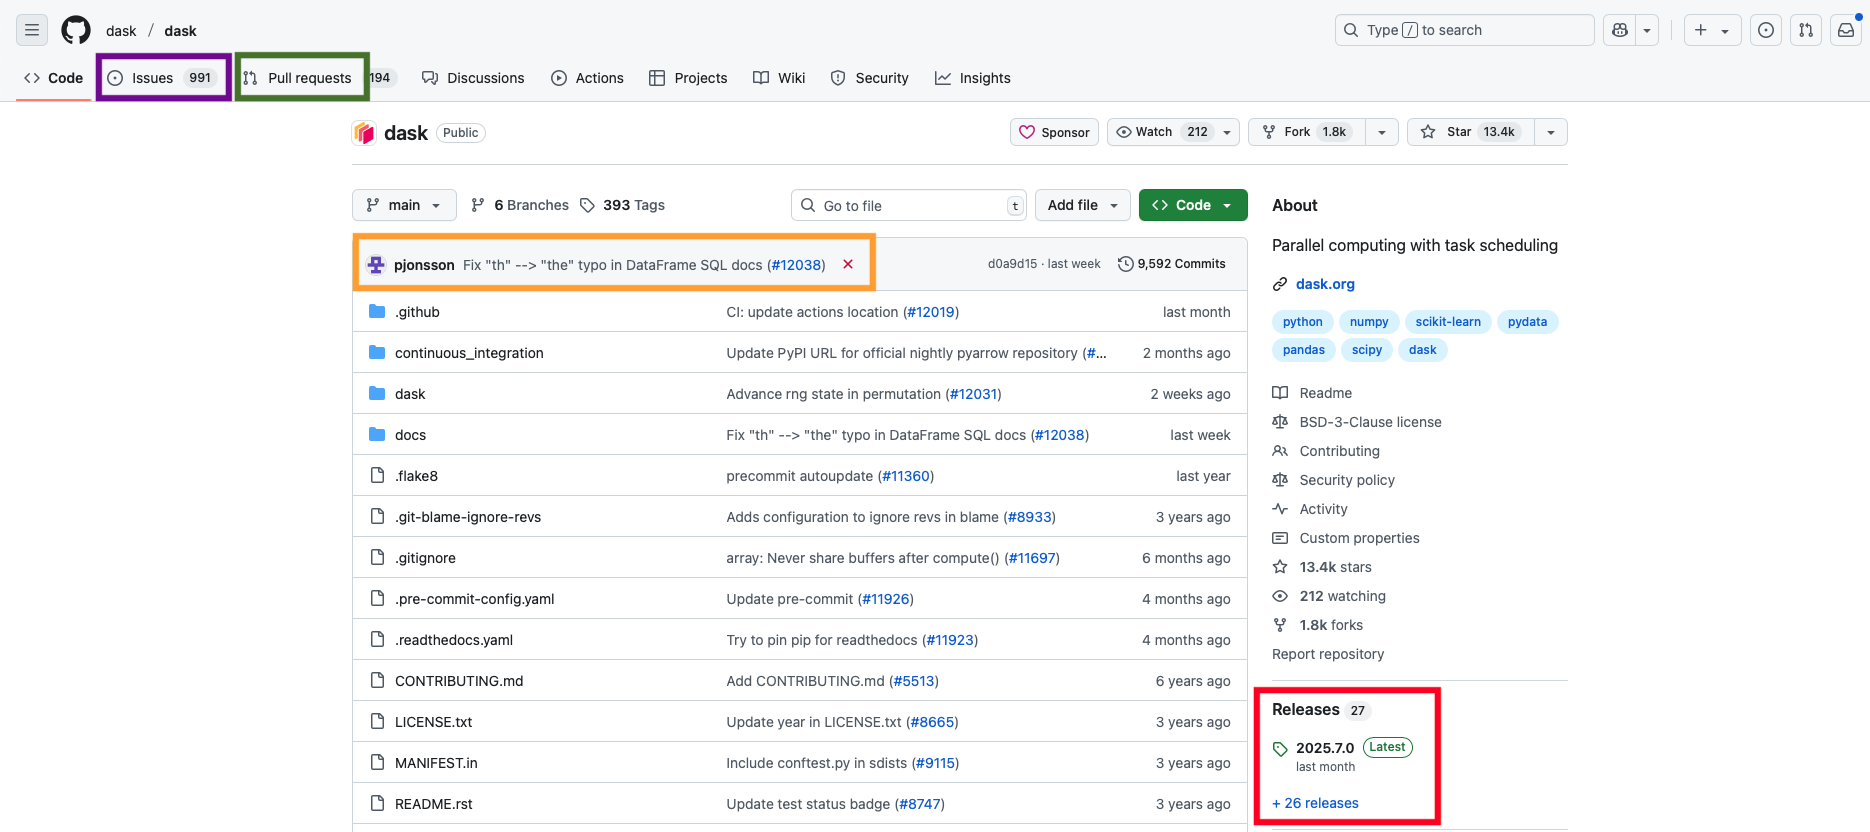
\includegraphics[width=\textwidth]{temp/dask_explainers/dask_homepage.png}
  \end{subfigure}

  \medskip

  \begin{subfigure}[b]{0.9\textwidth}
    \centering
    \caption{Example issue thread}\label{fig:dask-issue}
    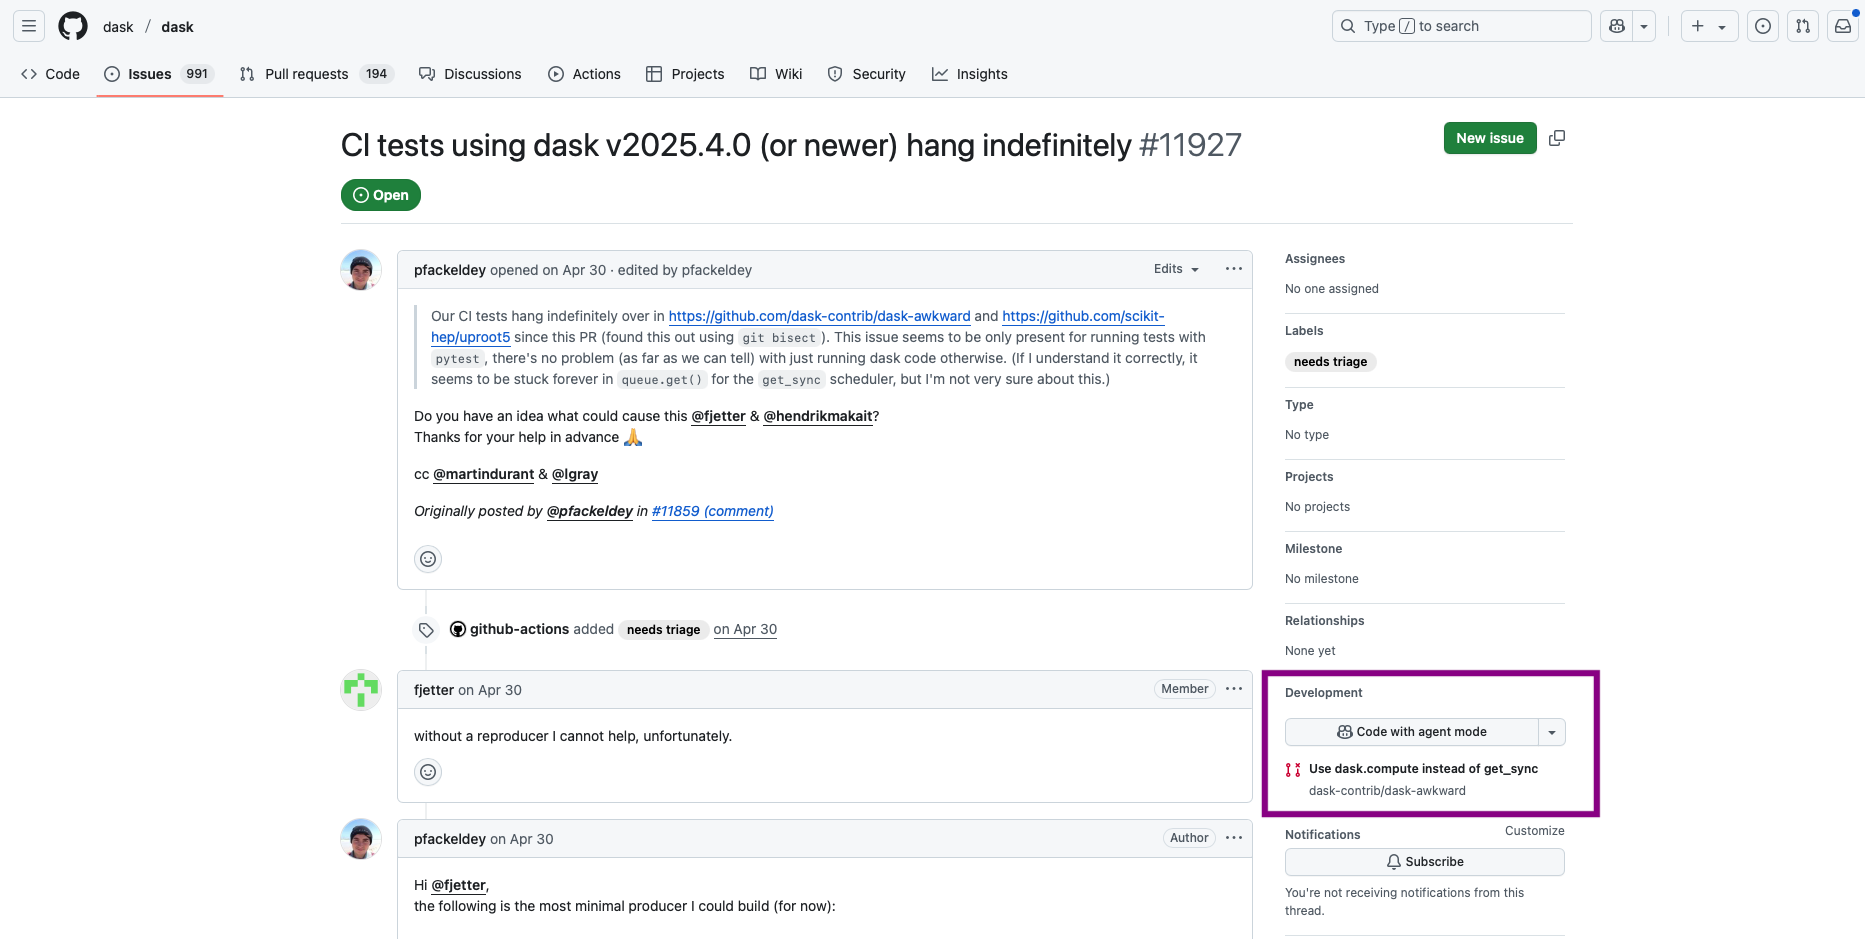
\includegraphics[width=\textwidth]{temp/dask_explainers/issue_thread.png}
  \end{subfigure}

    \bigskip
  \vspace{1ex}
  \centering
  \begin{minipage}{0.9\textwidth}
    \textbf{Figure notes:} 
    Panel~\subref{fig:dask-home} shows the \texttt{dask/dask} homepage (captured Aug 10, 12:21 PM EST).  
    The purple box links to unresolved issues (count shown); the green box links to open pull requests (count shown);  
    the orange box marks the most recent commit and its author; the red box highlights the latest release details. 
    Panel~\subref{fig:dask-issue} shows an issue thread, with the red box indicating the linked pull request. The issue was opened by user \textbf{pfackeldey} on April 30th, 2025 and received a response by \textbf{fjetter} that same day. 
  \end{minipage}

  \todo[inline]{Move to source/raw, improve title of figure}

\end{figure}
\pagebreak
\begin{figure}[ht]

    \caption{Descriptive statistics of key project metrics} \label{fig:summary-stats}
  
  \centering
  \medskip

  % Panel A
\begin{subfigure}[b]{0.9\textwidth}
  \centering
  \footnotesize
  \caption{Project summary statistics}
  \label{fig:project-summary-stats}
  \begin{tabular}{@{}l r *{5}{r}@{}}
    \toprule
    Metric                        & Mean   & \multicolumn{5}{c}{Percentiles} \\
    \cmidrule(lr){3-7}
                                  &        & 10th   & 25th   & 50th   & 75th   & 90th   \\
    \midrule
    Contributors                   & 106.72 & 9      & 20     & 49     & 120    & 239    \\
    Problems                       & 204.99 & 11     & 35     & 89     & 257    & 562    \\
    Unlinked issues                & 110.61 & 4      & 15     & 44     & 146    & 292    \\
    Unlinked pull requests         & 73.77  & 3      & 10     & 28     & 80     & 170    \\
    Linked issue–pull request pairs & 20.61  & 0      & 1      & 5      & 20     & 53     \\
    Discussions per problem        & 4.03   & 2      & 2.76   & 3.67   & 4.82   & 6.46   \\
    Contributors per problem       & 1.95   & 1.45   & 1.68   & 1.96   & 2.19   & 2.45   \\
    Time periods per project       & 13.86  & 8      & 10     & 15     & 18     & 18     \\
    \bottomrule
  \end{tabular}
\end{subfigure}

  \bigskip

  % Panel B
  \begin{subfigure}[b]{0.9\textwidth}
\caption{Contributor counts by filtering stage} \label{fig:departed-summary-stats}
    \centering
    \small
    \begin{tabular}{@{}p{0.65\textwidth} r@{}}
      \toprule
      Filter & \multicolumn{1}{c}{Contributors Remaining} \\
      \midrule
      All contributors                                    & 1,076,901 \\
      $\ge 3$ consecutive periods above 75th pct.\ commits &   13,773   \\
      Made 0 commits after departure                      &    7,646   \\
      In projects with only one departure                 &    1,594   \\
      Excluding departures from projects abandoned ≤ 3 periods later or contributors who remained active in the project &    262   \\
      In projects with $\ge 2$ important contributors     &       92   \\
      \bottomrule
    \end{tabular}
  \end{subfigure}
    \bigskip
  % Notes and overall caption
  \vspace{1ex}
  \begin{minipage}{0.9\textwidth}
    \small
    \textbf{Table Notes:}
    Panel~\subref{fig:project-summary-stats} presents the mean and selected percentiles (10th, 25th, 50th, 75th, 90th) for key project–period metrics: number of contributors, problems, unlinked issues, unlinked pull requests, linked issue–pull request pairs, discussions per problem, and contributors per problem. All statistics are based on project–time period observations. The last row includes the mean and selected percentiles for the number of periods each project appears in. 
    Panel~\subref{fig:departed-summary-stats} shows the number of contributors remaining after each filtering step.
  \end{minipage}


\end{figure}
\pagebreak

\begin{figure}[htbp]
    \centering
    \begin{minipage}[b]{0.49\textwidth}
        \centering
        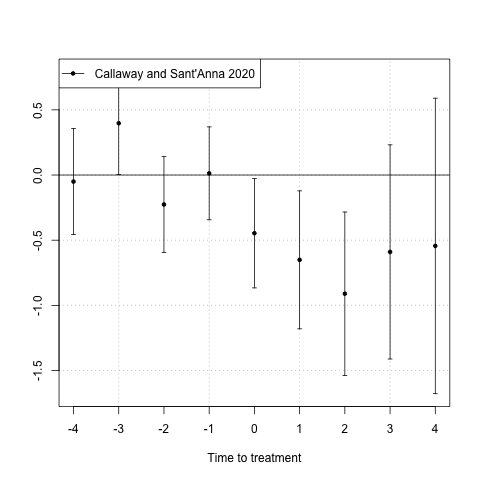
\includegraphics[width=\textwidth]{temp/output/prs_opened_norm.png}
        \subcaption{All projects}
        \label{fig:all_prs_opened}
    \end{minipage}
    \hfill
    \begin{minipage}[b]{0.49\textwidth}
        \centering
        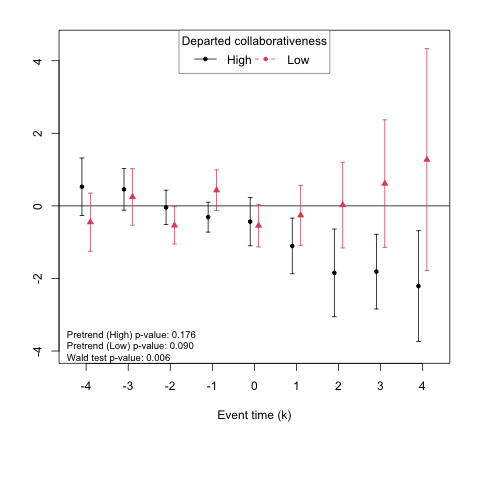
\includegraphics[width=\textwidth]{temp/output/collab/prs_opened_collab_cs_norm.png}
        \subcaption{By departed contributor collaborativeness}
        \label{fig:all_prs_opened_collab}
    \end{minipage}
    \caption{Impact of Key Contributor Departures on Project Outcomes}
    \label{fig:prs_opened}
\end{figure}

\begin{figure}[htbp]
    \caption{Subsetting by contributor join date}
    \label{fig}
    \centering
    \begin{minipage}[b]{0.49\textwidth}
        \centering
        \subcaption{Contributors who joined prior to departure} \label{fig}
        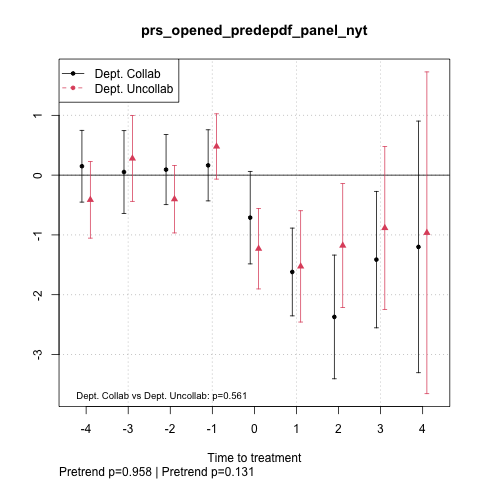
\includegraphics[width=\textwidth]{temp/output/collab/cs_norm_prs_opened_predep.png}
    \end{minipage}
    \hfill
    \begin{minipage}[b]{0.49\textwidth}
        \centering
        \subcaption{All contributors except the departed}\label{fig}
        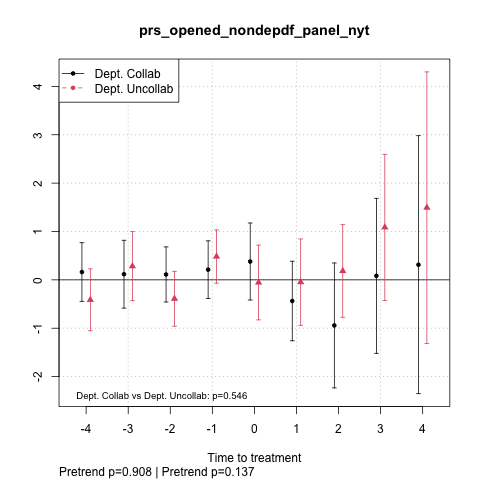
\includegraphics[width=\textwidth]{temp/output/collab/cs_norm_prs_opened_nondep.png}
    \end{minipage}


\todo[inline]{Graph improvements
1. Align axis for Panel a and b to -3.5 to 4.5 with ticks at every .5 (or 1)\\
2. Add figure notes describing definition of collaboration, confidence intervals (bootstrap 95 CI). \\
3. Change legend to indicate "Departed Contributor Collaborativeness" and have values be collaborative uncollaborative. \\
4. Remove grid background\\
5. Change time to treatment to "event time (k)"\\
6. Remove ugly bold label\\
7. Fine tune the plot subtitles
}

\end{figure}

\begin{figure}[htbp]
    \caption{Impact of Departures on Others by Extensive Margin Communication History}
    \label{fig:prs_opened_comm_ext_marg}
    \centering
        \begin{minipage}[b]{0.49\textwidth}
        \centering
        \subcaption{Highly collaborative} \label{fig:predep_prs_opened_high_collab_comm_ext_marg}
        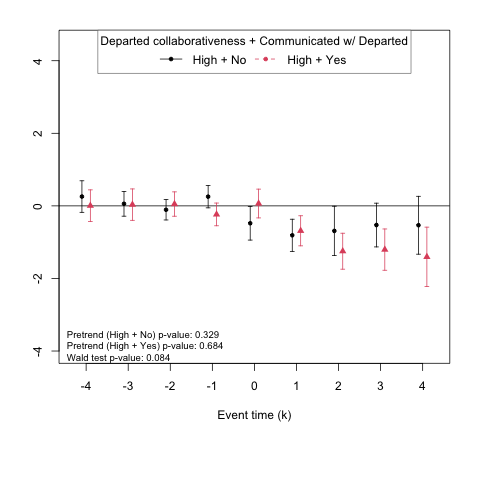
\includegraphics[width=\textwidth]{temp/output/collab/cs_norm_prs_opened_dept_never_comm_predep_High.png}
    \end{minipage}
    \hfill
    \label{fig:prs_opened_comm_ext_marg_low}
    \centering
        \begin{minipage}[b]{0.49\textwidth}
        \centering
        \subcaption{Less collaborative } \label{fig:predep_prs_opened_low_collab_comm_ext_marg}
        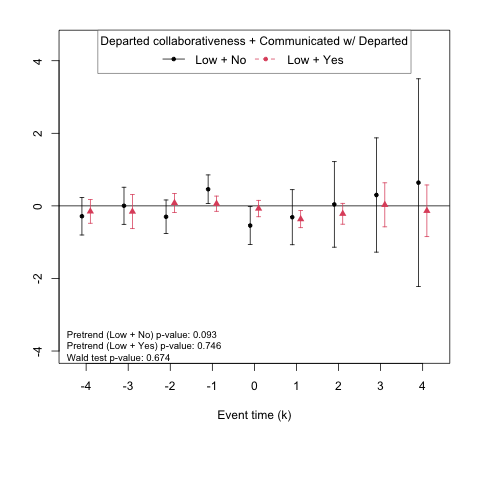
\includegraphics[width=\textwidth]{temp/output/collab/cs_norm_prs_opened_dept_never_comm_predep_Low.png}
    \end{minipage}
    
  \begin{minipage}{1\textwidth}
    \textbf{Figure notes:} 
    Following Callaway and Sant’Anna (2021), I estimate event-study coefficients accompanied by 95\% simultaneous confidence bands. For each plot with event study estimates from two subsamples, I report three Wald-test p-values: one for the pretrend test in the first subsample, one for the pretrend test in the second subsample (both from Equation \ref{eq:wald_test_pretrends} in Section \ref{sec:main_method}), and one for the difference in treatment effects across subsamples (Equation \ref{eq:wald_test} in Section \ref{sec:att_subset}). 
    Panel~\subref{fig:predep_prs_opened_high_collab_comm_ext_marg} replaces the standardized outcome’s total pull request count with that of two different member subsets: members who had ever \textbf{communicated with the departed} and members who had \textbf{never communicated with the departed} prior to estimation (as defined in Section~\ref{sec:contr_subset}) and conditions on organizations with highly collaborative departed members.
    Panel~\subref{fig:predep_prs_opened_low_collab_comm_ext_marg} is the analog of Panel~\subref{fig:predep_prs_opened_high_collab_comm_ext_marg} for less collaborative departed members.  
  \end{minipage}
  

\end{figure}

\begin{figure}[htbp]
    \caption{Subsetting by contributor communication intensity}
    \label{fig}
    \centering
    \begin{minipage}[b]{0.49\textwidth}
        \centering
        \subcaption{Communication (lifetime)} \label{fig}
        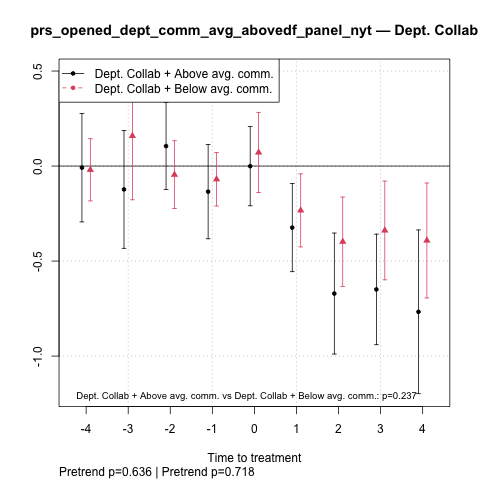
\includegraphics[width=\textwidth]{temp/output/collab/cs_norm_prs_opened_dept_comm_avg_above_Dept.Collab.png}
    \end{minipage}
    \hfill
    \begin{minipage}[b]{0.49\textwidth}
        \centering
        \subcaption{Communication per Problem}\label{fig}
        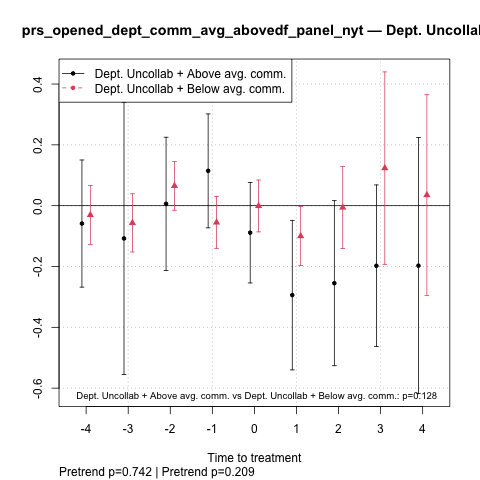
\includegraphics[width=\textwidth]{temp/output/collab/cs_norm_prs_opened_dept_comm_avg_above_Dept.Uncollab.png}
    \end{minipage}
        \begin{minipage}[b]{0.49\textwidth}
        \centering
        \subcaption{Communication (lifetime)} \label{fig}
        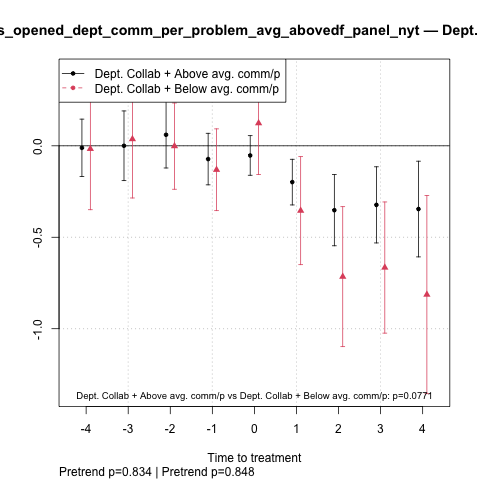
\includegraphics[width=\textwidth]{temp/output/collab/cs_norm_prs_opened_dept_comm_per_problem_avg_above_Dept.Collab.png}
    \end{minipage}
    \hfill
    \begin{minipage}[b]{0.49\textwidth}
        \centering
        \subcaption{Communication per Problem}\label{fig}
        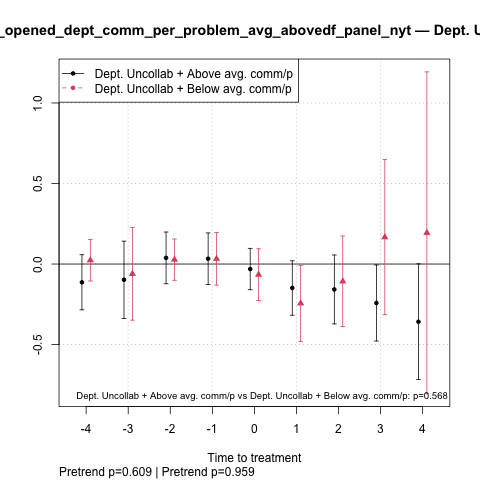
\includegraphics[width=\textwidth]{temp/output/collab/cs_norm_prs_opened_dept_comm_per_problem_avg_above_Dept.Uncollab.png}
    \end{minipage}


\todo[inline]{Graph improvements
1. Align axis for Panel a and b to -3.5 to 4.5 with ticks at every .5 (or 1)\\
2. Add figure notes describing definition of collaboration, confidence intervals (bootstrap 95 CI). \\
3. Change legend to indicate "Departed Contributor Collaborativeness" and have values be collaborative uncollaborative. \\
4. Remove grid background\\
5. Change time to treatment to "event time (k)"\\
6. Remove ugly bold label\\
7. Fine tune the plot subtitles
}

\end{figure}


\begin{figure}[htbp]   
    \caption{Impact of Departed Importance on Organizational Outcomes} \label{fig:prs_opened_more_imp}
    \centering
    \begin{minipage}[b]{0.49\textwidth}
        \centering
        \subcaption{By problem involvement}    \label{fig:prs_opened_involved}
        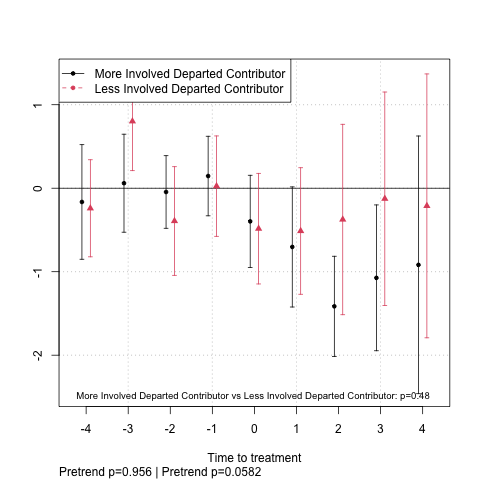
\includegraphics[width=\textwidth]{temp/output/collab/prs_opened_involved_cs_norm.png}
    \end{minipage}
    \begin{minipage}[b]{0.49\textwidth}
        \centering
        \subcaption{By PR opening involvement}    \label{fig:prs_opened_pr_involved}
        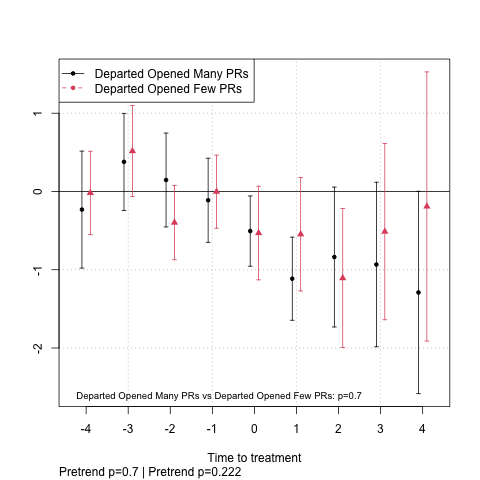
\includegraphics[width=\textwidth]{temp/output/collab/prs_opened_departed_opened_cs_norm.png}
    \end{minipage}
    \begin{minipage}[b]{0.49\textwidth}
        \centering
        \subcaption{More involved}    \label{fig:prs_opened_more_involved}
        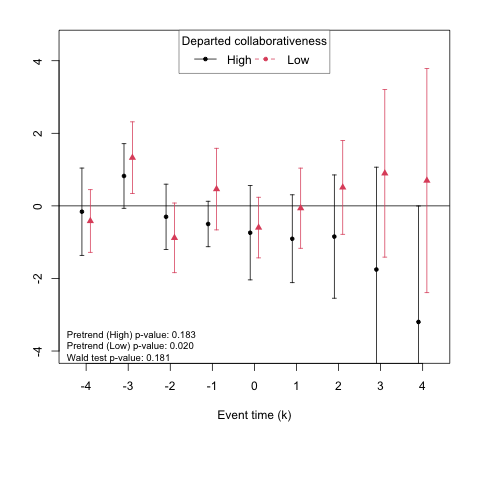
\includegraphics[width=\textwidth]{temp/output/collab_imp/inv0_cs_norm_prs_opened.png}
    \end{minipage}
    \begin{minipage}[b]{0.49\textwidth}
        \centering
        \subcaption{Less involved }    \label{fig:prs_opened_less_involved}
        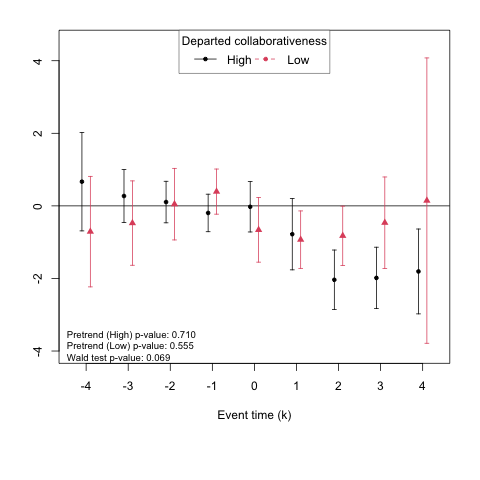
\includegraphics[width=\textwidth]{temp/output/collab_imp/inv1_cs_norm_prs_opened.png}
    \end{minipage}

  \begin{minipage}{1\textwidth}
    \textbf{Figure notes:} 
    Following Callaway and Sant’Anna (2021), I estimate event-study coefficients accompanied by 95\% simultaneous confidence bands. For each plot with event study estimates from two subsamples, I report three Wald-test p-values: one for the pretrend test in the first subsample, one for the pretrend test in the second subsample (both from Equation \ref{eq:wald_test_pretrends} in Section \ref{sec:main_method}), and one for the difference in treatment effects across subsamples (Equation \ref{eq:wald_test} in Section \ref{sec:att_subset}).  Panel~\subref{fig:prs_opened_involved}  subsets organizations by \textbf{departed member involvement}, as defined in Section~\ref{sec:org_level_subset}. Panel~\subref{fig:prs_opened_pr_involved}  subsets organizations by \textbf{departed member pull request involvement}, as defined in Section~\ref{sec:org_level_subset}. Panel~\subref{fig:prs_opened_more_involved} and Panel~\subref{fig:prs_opened_less_involved} condition on organizations where the departed was more and less involved by \textbf{departed member pull request involvement}, respectively and both subset by departed contributor collaborativeness
  \end{minipage}

\end{figure}

\begin{figure}[htbp]
    \centering
    % First row
    \begin{minipage}[b]{0.49\textwidth}
        \centering
        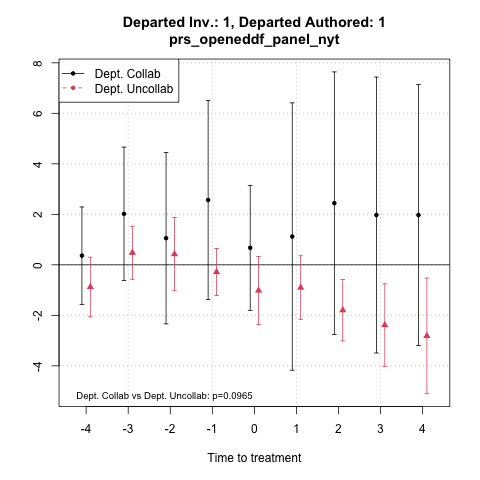
\includegraphics[width=\textwidth]{temp/output/collab_imp/auth1_inv1_cs_norm_prs_opened.png}
    \subcaption{Integral departed contributor}
    \label{fig:prs_opened_integral}
    \end{minipage}
    \hfill
    \begin{minipage}[b]{0.49\textwidth}
        \centering
        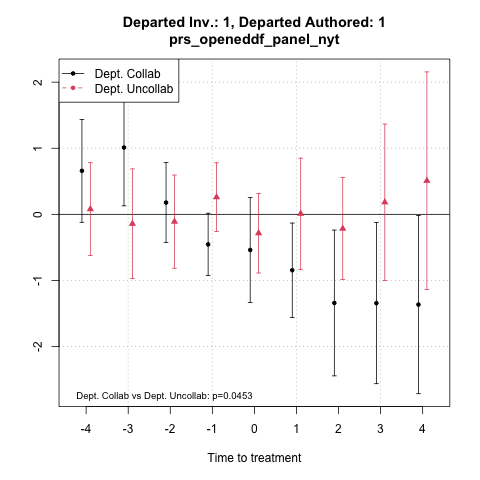
\includegraphics[width=\textwidth]{temp/output/collab_imp/auth_n1_inv_n1_cs_norm_prs_opened.png}
    \subcaption{Non-integral departed contributor}
    \label{fig:prs_opened_nonintegral}
    \end{minipage}

    
    \begin{minipage}[b]{0.32\textwidth}
        \centering
        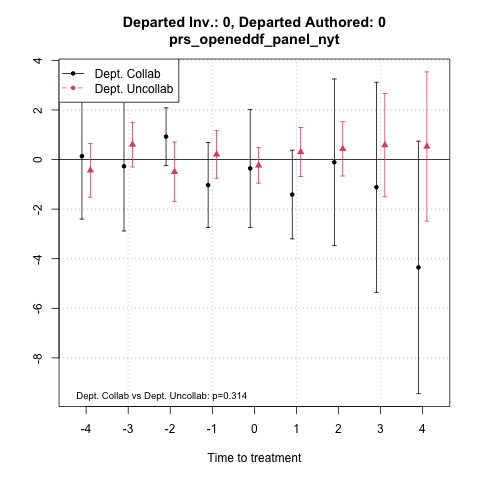
\includegraphics[width=\textwidth]{temp/output/collab_imp/auth0_inv0_cs_norm_prs_opened.png}
    \subcaption{Departed less involved, opened few PRs}
    \label{fig:prs_opened_noninv_nonopen}
    \end{minipage}
    \hfill
    \begin{minipage}[b]{0.32\textwidth}
        \centering
        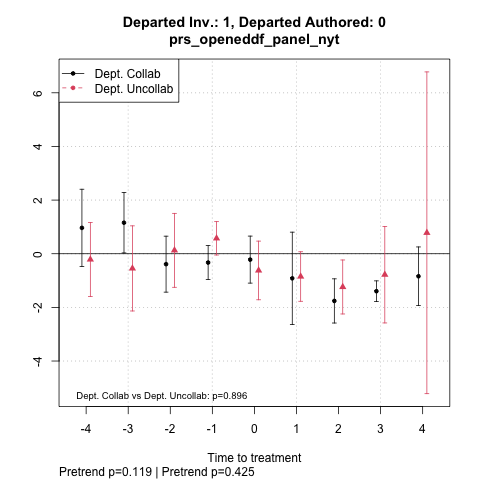
\includegraphics[width=\textwidth]{temp/output/collab_imp/auth0_inv1_cs_norm_prs_opened.png}
    \subcaption{Departed very involved, opened few PRs}
    \label{fig:prs_opened_inv_nonopen}
    \end{minipage}
    \hfill
    \begin{minipage}[b]{0.32\textwidth}
        \centering
        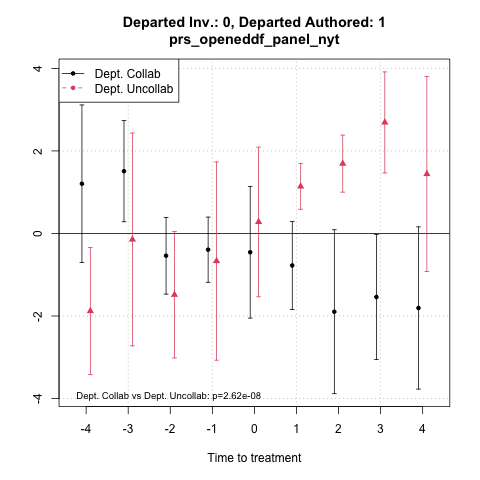
\includegraphics[width=\textwidth]{temp/output/collab_imp/auth1_inv0_cs_norm_prs_opened.png}
    \subcaption{Departed less involved, opened many PRs}
        \label{fig:prs_opened_nonvinv_open}

    \end{minipage}
    \caption{Departure Impact on Pull Requests Opened, by Departed Contributor Importance and Collaborativeness}
    \label{fig:prs_opened_inv_collab}
\end{figure}

\begin{figure}[htbp]
    \centering
    \begin{minipage}[b]{0.49\textwidth}
        \centering
        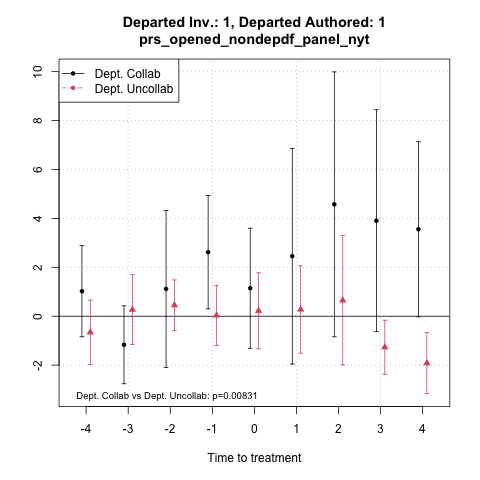
\includegraphics[width=\textwidth]{temp/output/collab_imp/auth1_inv1_cs_norm_prs_opened_nondep.png}
    \subcaption{All contributors except the departed}
    \label{fig:prs_opened_nondep}
    \end{minipage}
    \hfill
    \begin{minipage}[b]{0.49\textwidth}
        \centering
        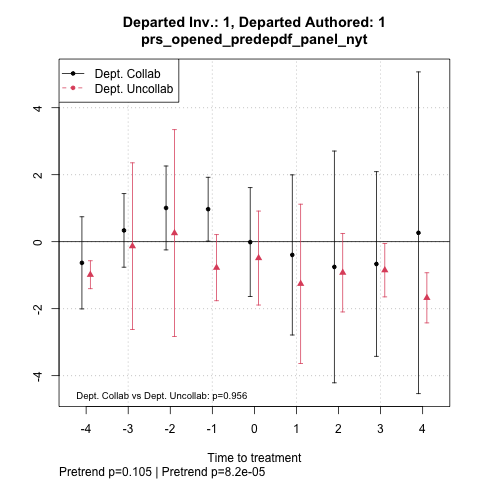
\includegraphics[width=\textwidth]{temp/output/collab_imp/auth1_inv1_cs_norm_prs_opened_predep.png}
    \subcaption{All contributors present prior to departure}
    \label{fig:prs_opened_predep}
    \end{minipage}
    \hfill
    \begin{minipage}[b]{0.49\textwidth}
        \centering
        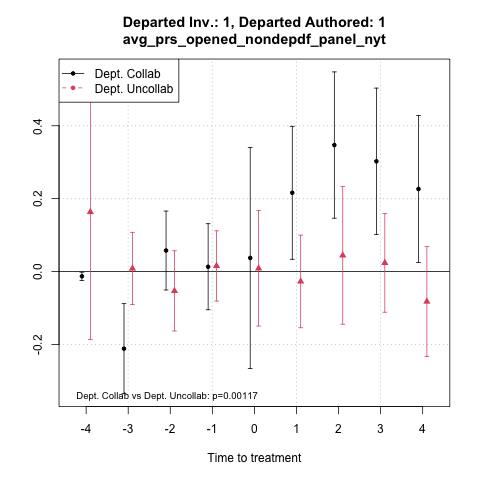
\includegraphics[width=\textwidth]{temp/output/collab_imp/auth1_inv1_cs_norm_avg_prs_opened_nondep.png}
    \subcaption{Average PRs opened, all but departed}
    \label{fig:avg_prs_opened_nondep}

    \end{minipage}
    \hfill
    \begin{minipage}[b]{0.49\textwidth}
        \centering
        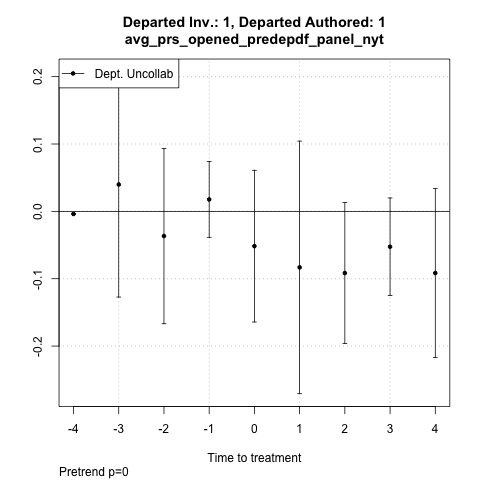
\includegraphics[width=\textwidth]{temp/output/collab_imp/auth1_inv1_cs_norm_avg_prs_opened_predep.png}
    \subcaption{Average PRs opened, contributors present pre-departure}
    \label{fig:avg_prs_opened_predep}
    \end{minipage}
    \hfill
    \begin{minipage}[b]{0.49\textwidth}
        \centering
        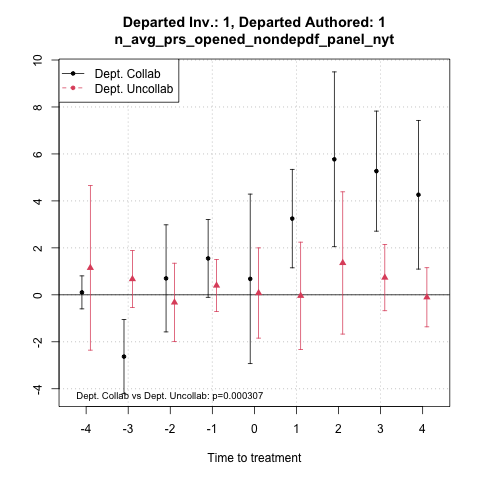
\includegraphics[width=\textwidth]{temp/output/collab_imp/auth1_inv1_cs_norm_n_avg_prs_opened_nondep.png}
    \subcaption{Impact of changes in average, all but departed}
    \label{fig:impact_avg_prs_opened_nondep}
    \end{minipage}
    \hfill
    \begin{minipage}[b]{0.49\textwidth}
        \centering
        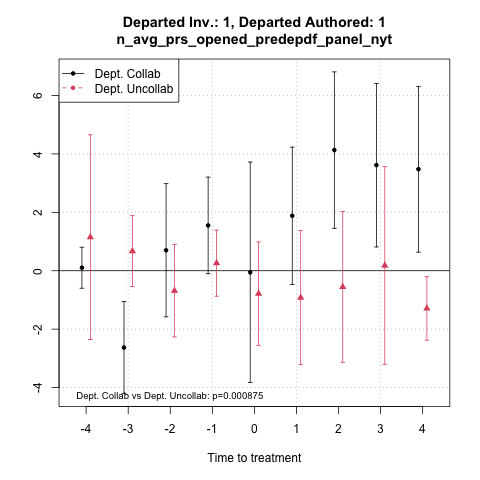
\includegraphics[width=\textwidth]{temp/output/collab_imp/auth1_inv1_cs_norm_n_avg_prs_opened_predep.png}
    \subcaption{Impact of changes in average, contirbutors present pre-departure}
    \label{fig:impact_avg_prs_opened_predep}

    \end{minipage}
    \caption{Integral Departure Impact on Average Outcomes and Participation}
\end{figure}

\begin{figure}[htbp]
    \centering
    \begin{minipage}[b]{0.49\textwidth}
        \centering
        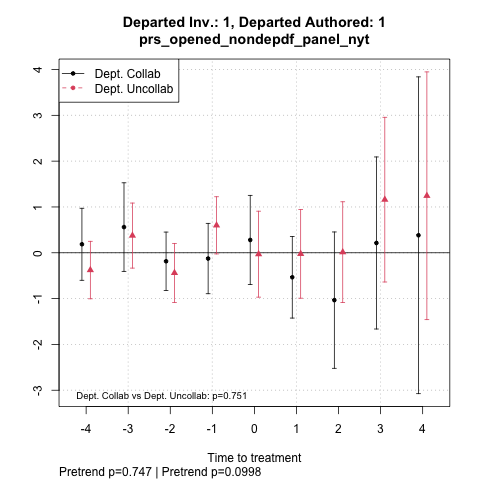
\includegraphics[width=\textwidth]{temp/output/collab_imp/auth_n1_inv_n1_cs_norm_prs_opened_nondep.png}
    \subcaption{All contributors except the departed}
    \end{minipage}
    \hfill
    \begin{minipage}[b]{0.49\textwidth}
        \centering
        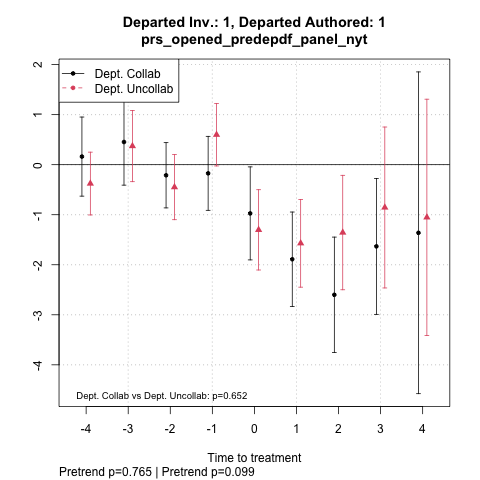
\includegraphics[width=\textwidth]{temp/output/collab_imp/auth_n1_inv_n1_cs_norm_prs_opened_predep.png}
    \subcaption{All contributors present prior to departure}
    \end{minipage}
    \hfill
    \begin{minipage}[b]{0.49\textwidth}
        \centering
        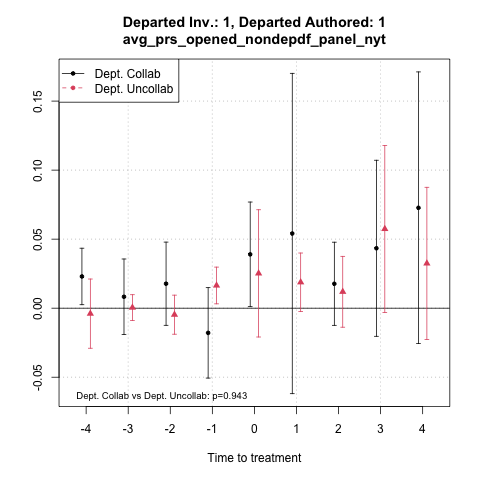
\includegraphics[width=\textwidth]{temp/output/collab_imp/auth_n1_inv_n1_cs_norm_avg_prs_opened_nondep.png}
    \subcaption{Average PRs opened, all but departed}
    \end{minipage}
    \hfill
    \begin{minipage}[b]{0.49\textwidth}
        \centering
        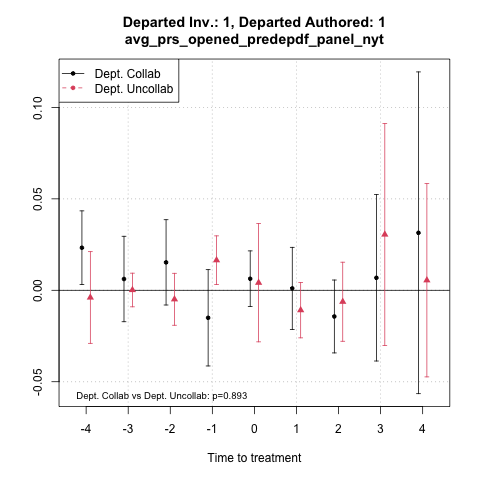
\includegraphics[width=\textwidth]{temp/output/collab_imp/auth_n1_inv_n1_cs_norm_avg_prs_opened_predep.png}
    \subcaption{Average PRs opened, contributors present pre-departure}
    \end{minipage}
    \hfill
    \begin{minipage}[b]{0.49\textwidth}
        \centering
        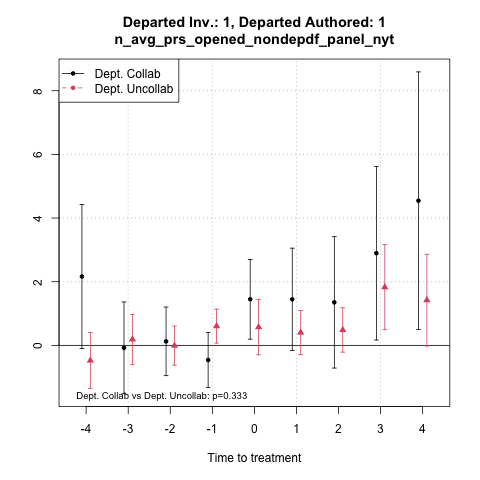
\includegraphics[width=\textwidth]{temp/output/collab_imp/auth_n1_inv_n1_cs_norm_n_avg_prs_opened_nondep.png}
    \subcaption{Impact of changes in average, all but departed}
    \end{minipage}
    \hfill
    \begin{minipage}[b]{0.49\textwidth}
        \centering
        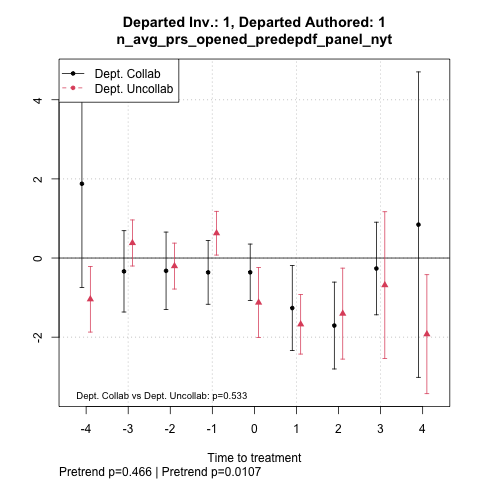
\includegraphics[width=\textwidth]{temp/output/collab_imp/auth_n1_inv_n1_cs_norm_n_avg_prs_opened_predep.png}
    \subcaption{Impact of changes in average, contirbutors present pre-departure}
    \end{minipage}
    \caption{Integral Departure Impact on Average Outcomes and Participation}
\end{figure}

\begin{figure}[htbp]
    \centering
    \begin{minipage}[b]{0.32\textwidth}
        \centering
        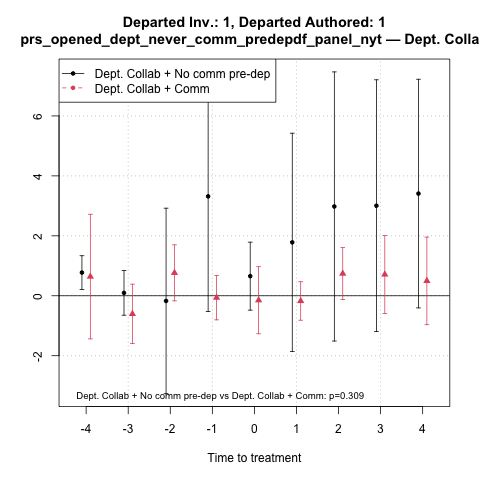
\includegraphics[width=\textwidth]{temp/output/collab_imp/auth1_inv1_cs_norm_prs_opened_dept_never_comm_predep_Dept.Collab.png}
    \subcaption{Communicators vs. Non-communicators, Collaborative Projects, integral departures}
    \label{fig:prs_opened_comm_collab_int_predep}
    \end{minipage}
    \hfill
    \begin{minipage}[b]{0.32\textwidth}
        \centering
        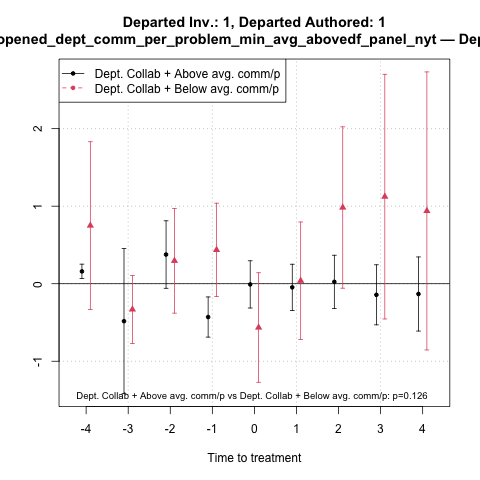
\includegraphics[width=\textwidth]{temp/output/collab_imp/auth1_inv1_cs_norm_prs_opened_dept_comm_per_problem_min_avg_above_Dept.Collab.png}
    \subcaption{Above vs. Below avg. communicators/problem, Collaborative Projects, integral departures}
    \label{fig:prs_opened_comm_collab_per_int}
    \end{minipage}
    \hfill
        \begin{minipage}[b]{0.32\textwidth}
        \centering
        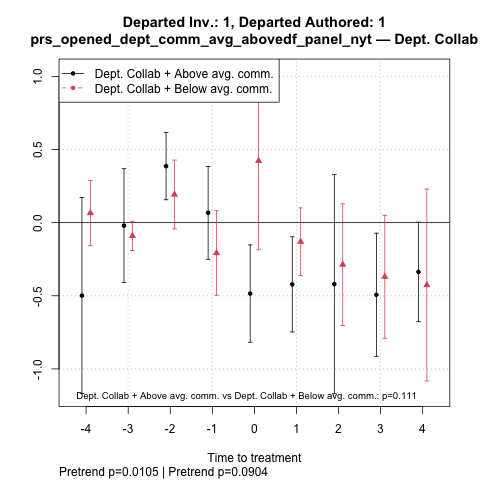
\includegraphics[width=\textwidth]{temp/output/collab_imp/auth1_inv1_cs_norm_prs_opened_dept_comm_avg_above_Dept.Collab.png}
    \subcaption{Above vs. Below avg. communicators, Collaborative Projects, integral departures}
    \label{fig:prs_opened_comm_collab_comm_int}
    \end{minipage}


    \begin{minipage}[b]{0.32\textwidth}
    \centering
    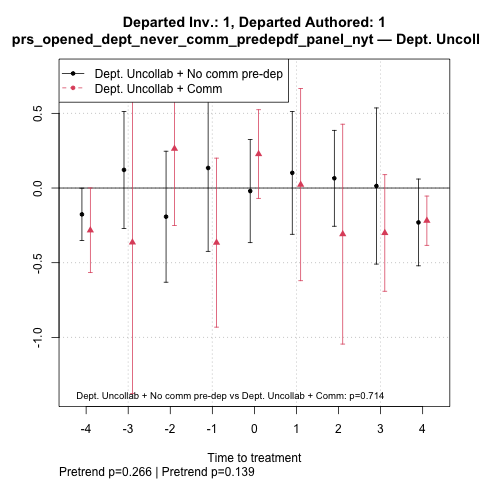
\includegraphics[width=\textwidth]{temp/output/collab_imp/auth1_inv1_cs_norm_prs_opened_dept_never_comm_predep_Dept.Uncollab.png}
    \subcaption{Communicators vs. Non-communicators, Uncollaborative Projects, integral departures}
    \label{fig:prs_opened_comm_uncollab_int_predep}
    \end{minipage}
    \hfill
    \begin{minipage}[b]{0.32\textwidth}
        \centering
        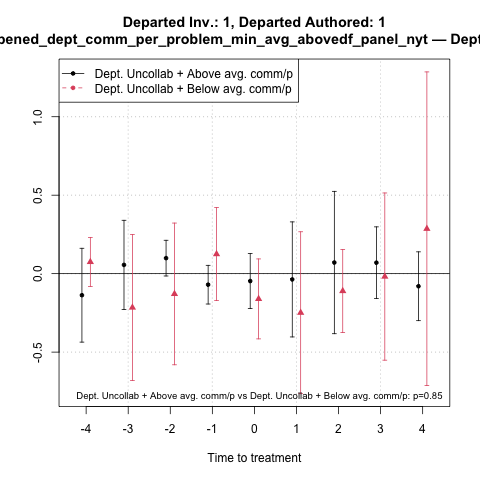
\includegraphics[width=\textwidth]{temp/output/collab_imp/auth1_inv1_cs_norm_prs_opened_dept_comm_per_problem_min_avg_above_Dept.Uncollab.png}
    \subcaption{Above vs. Below avg. communicators/problem, Uncollaborative Projects, integral departures}
    \label{fig:prs_opened_comm_uncollab_per_int}
    \end{minipage}
    \hfill
        \begin{minipage}[b]{0.32\textwidth}
        \centering
        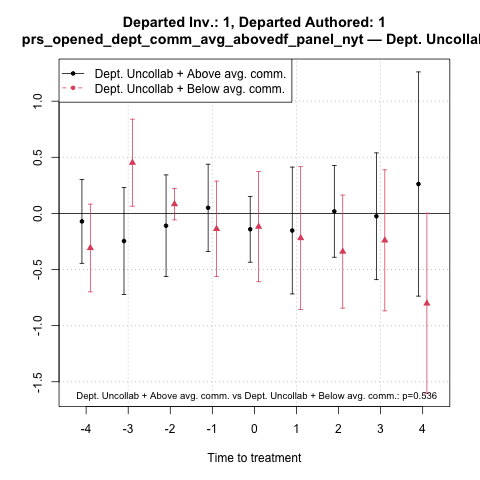
\includegraphics[width=\textwidth]{temp/output/collab_imp/auth1_inv1_cs_norm_prs_opened_dept_comm_avg_above_Dept.Uncollab.png}
    \subcaption{Above vs. Below avg. communicators, Uncollaborative Projects, integral departures}
    \label{fig:prs_opened_comm_uncollab_comm_int}
    \end{minipage}
    \caption{Impact of Communication on Post-Departure Outcomes in Projects with Integral Departures}
    \label{fig:prs_opened_comm}
\end{figure}

\begin{figure}[htbp]
    \centering
    \begin{minipage}[b]{0.24\textwidth}
        \centering
        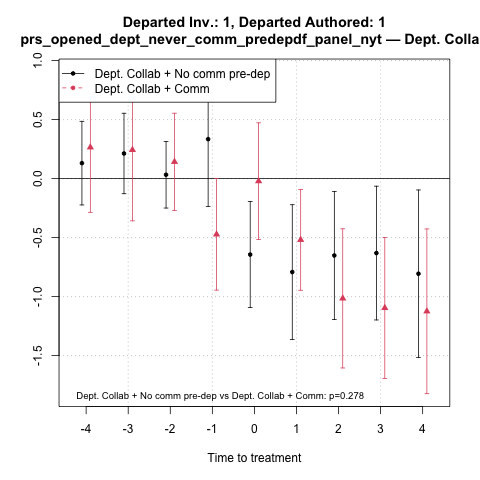
\includegraphics[width=\textwidth]{temp/output/collab_imp/auth_n1_inv_n1_cs_norm_prs_opened_dept_never_comm_predep_Dept.Collab.png}
    \subcaption{Communicators vs. Non-communicators, Collaborative Projects, integral departures}
    \label{fig:prs_opened_comm_collab_nonint_predep}
    \end{minipage}
    \hfill
    \begin{minipage}[b]{0.24\textwidth}
        \centering
        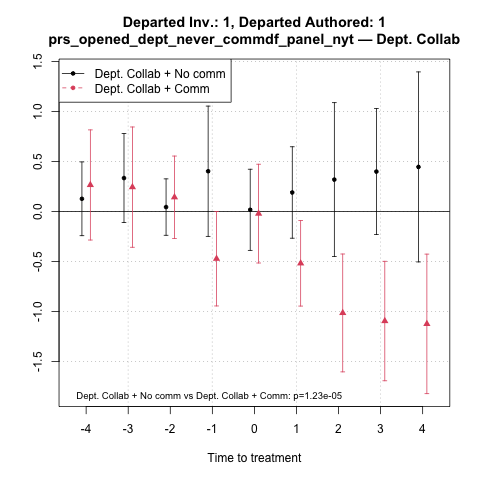
\includegraphics[width=\textwidth]{temp/output/collab_imp/auth_n1_inv_n1_cs_norm_prs_opened_dept_never_comm_Dept.Collab.png}
    \subcaption{Communicators vs. Non-communicators, Collaborative Projects, integral departures, include newcomers}
    \label{fig:prs_opened_comm_collab_nonint}
    \end{minipage}
    \hfill
    \begin{minipage}[b]{0.24\textwidth}
        \centering
        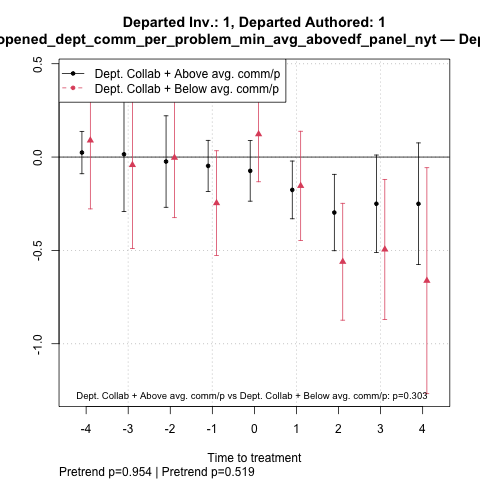
\includegraphics[width=\textwidth]{temp/output/collab_imp/auth_n1_inv_n1_cs_norm_prs_opened_dept_comm_per_problem_min_avg_above_Dept.Collab.png}
    \subcaption{Above vs. Below avg. communicators/problem, Collaborative Projects, integral departures}
    \label{fig:prs_opened_comm_collab_per_nonint}
    \end{minipage}
    \hfill
        \begin{minipage}[b]{0.24\textwidth}
        \centering
        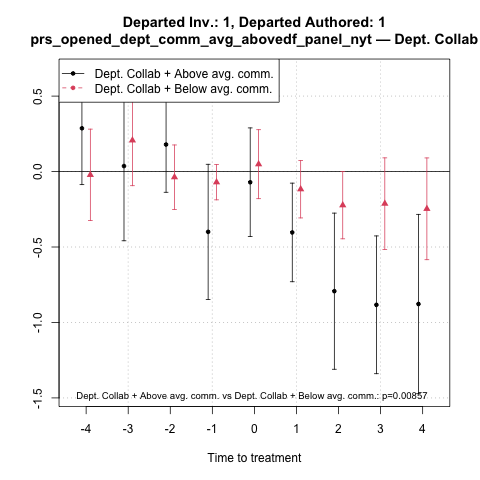
\includegraphics[width=\textwidth]{temp/output/collab_imp/auth_n1_inv_n1_cs_norm_prs_opened_dept_comm_avg_above_Dept.Collab.png}
    \subcaption{Above vs. Below avg. communicators, Collaborative Projects, integral departures}
    \label{fig:prs_opened_comm_collab_comm_nonint}
    \end{minipage}


    \begin{minipage}[b]{0.24\textwidth}
    \centering
    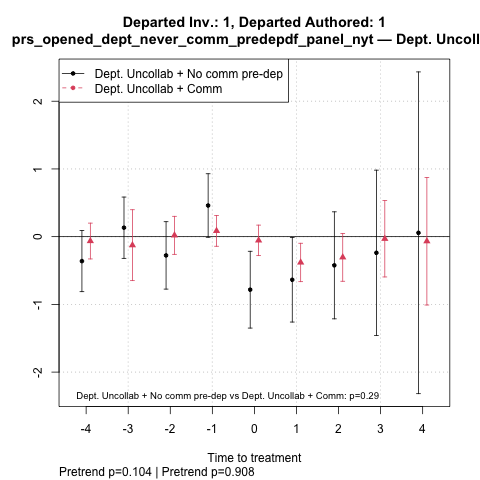
\includegraphics[width=\textwidth]{temp/output/collab_imp/auth_n1_inv_n1_cs_norm_prs_opened_dept_never_comm_predep_Dept.Uncollab.png}
    \subcaption{Communicators vs. Non-communicators, Uncollaborative Projects, integral departures}
    \label{fig:prs_opened_comm_uncollab_nonint_predep}
    \end{minipage}
    \hfill
    \begin{minipage}[b]{0.24\textwidth}
        \centering
        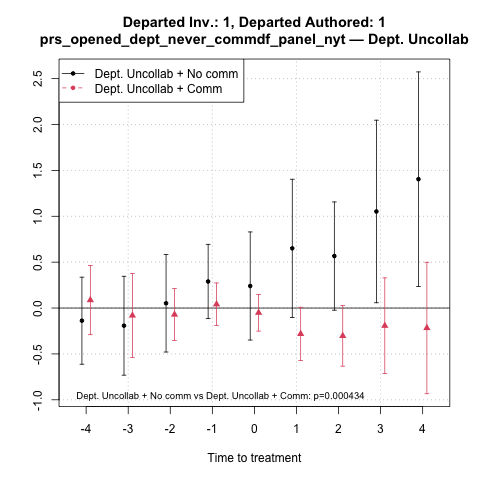
\includegraphics[width=\textwidth]{temp/output/collab_imp/auth_n1_inv_n1_cs_norm_prs_opened_dept_never_comm_Dept.Uncollab.png}
    \subcaption{Communicators vs. Non-communicators, Unollaborative Projects, integral departures, include newcomers}
    \label{fig:prs_opened_comm_collab_nonint}
    \end{minipage}
    \hfill
    \begin{minipage}[b]{0.24\textwidth}
        \centering
        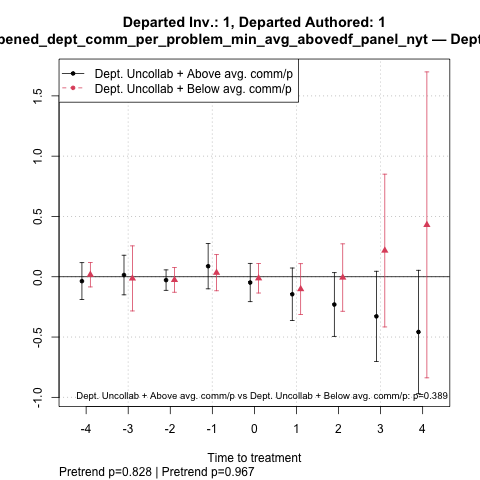
\includegraphics[width=\textwidth]{temp/output/collab_imp/auth_n1_inv_n1_cs_norm_prs_opened_dept_comm_per_problem_min_avg_above_Dept.Uncollab.png}
    \subcaption{Above vs. Below avg. communicators/problem, Uncollaborative Projects, integral departures}
    \label{fig:prs_opened_comm_uncollab_per_nonint}
    \end{minipage}
    \hfill
        \begin{minipage}[b]{0.24\textwidth}
        \centering
        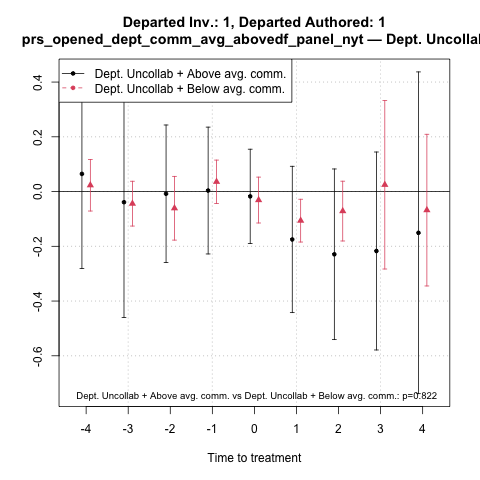
\includegraphics[width=\textwidth]{temp/output/collab_imp/auth_n1_inv_n1_cs_norm_prs_opened_dept_comm_avg_above_Dept.Uncollab.png}
    \subcaption{Above vs. Below avg. communicators, Uncollaborative Projects, integral departures}
    \label{fig:prs_opened_comm_uncollab_comm_nonint}
    \end{minipage}
    \caption{Impact of Communication on Post-Departure Outcomes in Projects with Integral Departures}
    \label{fig:prs_opened_comm}
\end{figure}




\clearpage

\onehalfspacing

\section*{Tables} \label{sec:tab}
\addcontentsline{toc}{section}{Tables}



\clearpage

\section*{Figures} \label{sec:fig}
\addcontentsline{toc}{section}{Figures}



\clearpage

\section*{Appendix A. Placeholder} \label{sec:appendixa}



\begin{itemize}
    \item Appendix: How I map PyPi projects to github repositories
    \item Appendix: How I match repo names to repo ids in cases where identity changes
    \item Appendix: How are commits measured and deal with the fact that push and PR commits can be overlapping? 
    \item Appendix: Robustness to 3 month measurements (if necessary)
\end{itemize}
\subsubsection{Defining the set of problems (the linking process)}
\begin{enumerate}
    \item First construct a mapping between issues + PRs. This helps create a dataset of "problems" that projects address
    \begin{itemize}
        \item Three problem types: unlinked issues, unlinked PRs, linked
        \item Construct linkage using the following criteria
        \begin{enumerate}
          \item Use the provided link.
          \item For each remaining unlinked issue/PR, find a counterpart that mutually references it and choose the closest number.
          \item If no mutual reference exists, find any one-way reference and choose the closest number
        \end{enumerate}
    \end{itemize}
    \item Only keep projects that have at least two important contributors in all pre-treatment periods (henceforth known as pre periods)
\end{enumerate}
\subsection{If this comes up, define other outcomes}


\begin{enumerate}
    \item Measurement of downstream outcomes - the deifne the ones that I end up using. 
    \item Describe software releases, the various types and measurement
    \item Define software quality (security measure, not user experience based)
    \item Downloads
\end{enumerate}

\subsection{Aspirational To Dos for data section }
\begin{enumerate}
    \item Read this  \href{https://pubs.aeaweb.org/doi/pdfplus/10.1257/jep.36.3.211}{paper} in order to understand how to motivate the paper using descriptive statistics
    \item Provide insight into what a project is like, such as
    \begin{itemize}
        \item What are churn rates like among both hierarchies?
        \item Provide estimates of data coverage at a project level     
    \end{itemize}
    \item Add reference to showing that results are not sensitive to changes in parameters/if they are, justify why mine is reasonable 
\end{enumerate}

\end{document}